\chapter{Analisis}
\label{chap:analisis}

Bab ini membahas tentang analisis kebutuhan \textit{Sharif Judge} yang diperlukan oleh Teknik Informatika dan solusi yang ditawarkan untuk memenuhi kebutuhan tersebut. Kebutuhan-kebutuhan tersebut didapat dari daftar isu repositori \textit{Sharif Judge} di \textit{GitHub} dan dari para dosen pengguna \textit{Sharif Judge}. Hasil dari analisis kebutuhan tersebut dicatat ke dalam \textit{Google Sheets} dan didiskusikan dengan dosen pembimbing. Selain analisis kebutuhan, pada bab ini juga akan dibahas analisis sistem kini pada perangkat lunak \textit{Sharif Judge}.


\section{Analisis Kebutuhan Perangkat Lunak \textit{Sharif Judge}}
\label{sec:analisis}
Analisis dilakukan dengan menganalisis setiap isu terbuka yang ada pada repositori di \textit{GitHub}. Setiap isu di \textit{GitHub} terdapat kode unik yang dimulai dengan tanda '\#' dan diikuti dengan angka. Kode unik tersebut menunjukan urutan isu yang dibuat oleh para pengguna \textit{GitHub}. Dari analisa setiap isu yang ada, didapatkan beberapa pertanyaan dan usulan pengembangan. Beberapa isu yang memiliki usulan pengembangan akan dijadikan pertimbangan untuk mengembangkan \textit{Sharif Judge}. \\

Analisis kebutuhan dari para dosen pengguna \textit{Sharif Judge} dilakukan dalam bentuk wawancara secara langsung dan melalui \textit{email}. Dosen-dosen yang telah diwawancarai antara lain:
\begin{enumerate}
	\item Husnul Hakim
	\item Claudio Franciscus
	\item Vania Natali
	\item Luciana Abednego
	\item Joanna Helga
\end{enumerate}
%Dari hasil wawancara didapatkan beberapa kebutuhan yang sama dari setiap dosen pengguna \textit{Sharif Judge}. 

\begin{table}[H] %atau h saja untuk "kira kira di sini"
	\centering 
	\caption{Tabel Analisis Kebutuhan \textit{Sharif Judge}}
	\label{tab:kebutuhan}
	\resizebox{\textwidth}{!}{%
	\begin{tabular}{|l|l|l|l|l|l|}
		\toprule
		No & Deskripsi & Sumber & \thead{\textit{Issue Number /} \\ Nama Mata Kuliah} & \thead{Pembuat \textit{Issue} \\ Nama Dosen} & Status\\
		
		\midrule
		1 & \textit{Security with PHP} & \textit{GitHub} & \#61 & kathiedart & Diimplemntasi\\ \hline
		2 & \textit{Securing Assignment}  & \textit{GitHub} & \#55 & wojcik13 & Tidak diimplementasi\\ \hline
		3 & \textit{New Function} & \textit{GitHub} & \#53 & wojcik13 & Tidak diimplementasi\\ \hline
		4 & \textit{Solved Problem Indicator} & \textit{GitHub} & \#46 & atiabjobayer & Tidak diimplementasi\\ \hline
		5 & \textit{Some Problem} \& \textit{Sugestion} & \textit{GitHub} & \#45 & atiabjobayer & Tidak diimplementasi\\ \hline
		6 & \makecell[l]{\textit{Queue failed to process if }\\\textit{ submission take too long to} \\ \textit{complete?}}  & \textit{GitHub} & \#32 & truongan & Diimplemntasi\\ \hline
		
		7 & \textit{Compilation Error on all language} & GitHub & \#34 & Eririn07 & Tidak diimplementasi\\ \hline
		8 & \makecell[l]{Membatasi soal (deskripsi dan PDF) \\ hanya bisa diakses saat \textit{assignment} \\ "\textit{open}" dan setelah waktu mulai} & Dosen & AIF102 & Husnul Hakim & Diimplementasi\\ \hline
		
		9 & \makecell[l]{Menguji kemiripan kode antar \\ mahasiswa (Contek)} & Dosen & AIF102 & Husnul Hakim & Tidak diimplementasi\\ \hline
		10 & \makecell[l]{1 Akun hanya dapat \textit{login} 1 waktu \\ (Jika suatu akun sedang \textit{login}, tidak \\ ada lagi yang bisa \textit{login} akun tersebut)} & Dosen & AIF102 & Husnul Hakim & Diimplementasi\\ \hline
		11 & \makecell[l]{Membatasi soal (deskripsi dan PDF) \\ hanya bisa diakses saat \textit{assignment} \\ "\textit{open}" dan setelah waktu mulai} & Dosen & AIF102 & Vania Natali & Diimplementasi\\ \hline
		12 & \makecell[l]{\textit{Sharif Judge} tidak dapat menerima \\ \textit{file} dengan ekstensi *.txt \\ untuk \textit{Pre-Test}} & Dosen & AIF102 & Vania Natali & Diimplementasi\\ \hline
		13 & \makecell[l]{Membatasi soal (deskripsi dan PDF) \\ hanya bisa diakses saat \textit{assignment} \\ "\textit{open}" dan setelah waktu mulai} & Dosen & AIF202 & Luciana Abednego & Diimplementasi\\ \hline
		14 & \makecell[l]{\textit{Sharif Judge} tidak dapat menerima \\ \textit{file} dengan ekstensi *.txt \\ untuk \textit{Pre-Test}} & Dosen & AIF202 & Luciana Abednego & Diimplementasi\\ \hline
		15 & \makecell[l]{Perlu ditambah petunjuk penamaan \\ \textit{file} \textit{input} \& \textit{output} yg langsung \\ bisa dilihat ketika hendak \textit{upload}} & Dosen & AIF202 & Luciana Abednego & Tidak diimplementasi\\ \hline
		16 & \makecell[l]{Membatasi soal (deskripsi dan PDF) \\ hanya bisa diakses saat \textit{assignment} \\ "\textit{open}" dan setelah waktu mulai} & Dosen & AIF202 & Joanna Helga & Diimplementasi\\ \hline
		17 & \makecell[l]{\textit{Register} peserta yg \textit{mode batch}, \\ \textit{Sharif Judge} tidak minta nama \\ orangnya (lebih baik ada nama orangnya)} & Dosen & AIF202 & Joanna Helga & Diimplementasi\\ \hline
		18 & \makecell[l]{Nama peserta seharusnya tidak \\ bisa diganti (Bisa menjadi \\ "mainan" dan tindak kecurangan \\ karena dapat memberikan \textit{hint})} & Dosen & AIF202 & Joanna Helga & Diimplementasi\\ \hline
		19 & \makecell[l]{Ingin memiliki fungsi dimana \\ \textit{Assignment} tidak memiliki batasan \\ waktu (arsip soal tahun \\ lalu dapat dikerjakan kapan saja)} & Dosen & AIF202 & Joanna Helga & Diimplementasi\\ \hline
		20 & \makecell[l]{Ingin memiliki \textit{scoreboard global} \\ untuk semua \textit{assignment}.} & Dosen & AIF202 & Joanna Helga & Diimplementasi\\ \hline
		21 & \makecell[l]{Membatasi soal (deskripsi dan PDF) \\ hanya bisa diakses saat \textit{assignment} \\ "\textit{open}" dan setelah waktu mulai} & Dosen & AIF102 \& AIF202 & Claudio Fransiscus & Diimplementasi\\ \hline
		22 & \makecell[l]{\textit{Sharif Judge} tidak dapat menerima \\ \textit{file} dengan ekstensi *.txt \\ untuk \textit{Pre-Test}} & Dosen & AIF102 \& AIF202 & Claudio Fransiscus & Diimplementasi\\ \hline
		23 & \makecell[l]{UI masih merepotkan} & Dosen & AIF102 \& AIF202 & Claudio Fransiscus & Tidak diimplementasi\\ \hline
		24 & \makecell[l]{UI ada yang tidak berguna \\ (yang lebih banyak digunakan \\ \textit{assignment, submit, scoreboard,} \\ dan hasil \textit{submit}} & Dosen & AIF102 \& AIF202 & Claudio Fransiscus & Tidak diimplementasi\\

		\bottomrule
		
	\end{tabular}}
\end{table}

\begin{table}[H] %atau h saja untuk "kira kira di sini"
	\centering 
	%\caption{\textit{Kebutuhan \textit{Sharif Judge}}}
	\label{tab:kebutuhan2}
	\resizebox{\textwidth}{!}{%
		\begin{tabular}{|l|l|l|l|l|l|}
			\hline
			25 & \makecell[l]{Ingin memiliki fungsi \textit{reminder}. \\ Banyak mahasiswa lupa mengerjakan \\ tugas dan tidak bisa mengumpulkan. \\ Fungsi \textit{reminder} akan mengirimkan \\ \textit{reminder} ke \textit{email} mahasiswa} & Dosen & AIF102 \& AIF202 & Claudio Fransiscus & Tidak diimplementasi\\ \hline
			26 & \makecell[l]{Membatasi soal (deskripsi dan PDF) \\ hanya bisa diakses saat \textit{assignment} \\ "\textit{open}" dan setelah waktu mulai} & Dosen & AIF102 \& AIF202 & Pascal Alfadian & Diimplementasi\\ \hline
			27 & \makecell[l]{Integrasi login ke \textit{RADIUS} \\ (\textit{password} sama dengan \textit{login Windows})} & Dosen & AIF401 & Pascal Alfadian & Diimplementasi\\ \hline
			28 & \makecell[l]{Mengumpulkan \textit{file} TXT} & Dosen & AIF401 & Pascal Alfadian & Diimplementasi\\ \hline
			29 & \makecell[l]{Mengumpulkan \textit{file} JAR (java multi kelas)} & Dosen & AIF401 & Pascal Alfadian & Tidak diimplementasi\\ \hline
			30 & Branding Teknik Informatika & Dosen & AIF401 & Pascal Alfadian & Diimplementasi\\ \hline
			31 & \makecell[l]{Download \textit{Excel} tidak berfungsi \\ pada halaman \textit{Submission}} & Asisten Dosen & AIF202 & Kresna Dwi Cahyo & Diimplementasi\\ \hline
	\end{tabular}}
\end{table}


Pada tabel di atas teradapat beberapa kolom, yaitu:
\begin{itemize}
	\item Deskripsi \\
	Jika sumber kebutuhan berasal dari \textit{GitHub}, maka pada kolom deskripsi akan ditulis judul dari isu yang ada pada repositori. Jika sumber kebutuhan berasal dari dosen, maka deskripsi kebutuhan langsung ditulis pada kolom tersebut.
	\item Sumber \\
	Kolom sumber berisikan sumber dari kebutuhan pengembangan \textit{Sharif Judge} yaitu \textit{GitHub} atau Dosen.
	\item \textit{Issue Number} / Nama Mata Kuliah \\
	Jika sumber kebutuhan berasal dari \textit{GitHub}, maka pada kolom ini akan ditulis \hyperref[sec:analisis]{kode unik} yang ada pada setiap isu. Jika sumber kebutuhan berasal dari dosen, maka pada kolom ini akan ditulis mata kuliah yang diajar oleh dosen tersebut. Keterangan kode mata kuliah AIF102 = Algoritma \& Struktur Data, AIF202 = Desain \& Analisis Algoritma dan AIF401 = Skripsi 1.
	\item Pembuat \textit{Issue} / Nama Dosen \\
	Jika sumber kebutuhan berasal dari \textit{GitHub}, maka pada kolom ini akan ditulis \textit{username} pembuat isu tersebut. Jika sumber kebutuhan berasal dari dosen, maka pada kolom ini akan ditulis nama dosen yang memberikan daftar kebutuhan.
	\item Status \\
	Kolom Status berisikan status dari kebutuhan tersebut apakah akan diimplementasi atau tidak diimplementasi.
\end{itemize}

%Pada tabel di atas terdapat kolom Deskirpsi, Sumber, Issue Number / Nama Mata Kuliah, Pembuat Issue / Nama Dosen dan Status. Kolom Deskripsi berisikan deskripsi kebutuhan yang disebutkan oleh para dosen, namun jika sumber kebutuhan berasal dari GitHub maka akan berisikan judul isu. Kolom Sumber berisikan sumber kebutuhan yaitu GitHub atau Dosen. Kolom Issue Number / Nama Mata Kuliah berisikan 

\subsection{\textit{Security with PHP}}
Isu dengan kode unik \#61 dibuat oleh pengguna \textit{GitHub} dengan username \textit{danwdart} pada tanggal 6 April 2017. Pada isu tersebut dikatakan bahwa seseorang pengguna \textit{Sharif Judge} dapat mengubah parameter \textit{PHP} \textit{shell\_exec(rm ...)} yang mengakibatkan pengeksekusian kode bisa dilakukan secara sewenang-wenang. Untuk menghindari hal di atas, username \textit{danwdart} menyarankan untuk mengganti perintah \textit{PHP} \textit{shell\_exec(rm ...)} dengan method lain.

Pada skripsi ini, isu di atas diimplementasi. Solusi yang ditawarkan adalah mengganti penggunaan \textit{PHP} \textit{shell\_exec(rm ...)} dengan \textit{method} lain.  Perintah \textit{shell\_exec("rm ...")} memiliki fungsi untuk menghapus sebuah file. Perintah tersebut dapat diganti menggunakan \textit{method} \textit{unlink()} yang memiliki fungsi sama yaitu menghapus sebuah file.
%Hal tersebut dapat dicegah dengan cara mengubah perintah shell\_exec("rm ...") dengan method \textit{unlink()}.

\subsection{\textit{Securing Assignment}}
Isu dengan kode unik \#55 dibuat oleh pengguna \textit{GitHub} dengan username \textit{wojcik13} pada tanggal 23 Oktober 2016. \textit{Username} \textit{wojcik13} menanyakan apakah ada pilihan pada \textit{Sharif Judge} untuk mengamankan assignment dengan password.

Pada skripsi ini, isu di atas tidak diimplementasi. Isu di atas merupakan sebuah pertanyaan fitur pada \textit{Sharif Judge} untuk mengamankan assignment dengan menggunakan password. Oleh karena isu tersebut merupakan sebuah pertanyaan, maka pada skripsi ini isu di atas tidak diimplementasi.

\subsection{\textit{New Function}}
Isu dengan kode unik \#53 dibuat oleh pengguna \textit{GitHub} dengan username \textit{wojcik13} pada tanggal 2 Oktober 2016. \textit{Username} \textit{wojcik13} menanyakan apakah ada fungsi pada \textit{Sharif Judge} seperti menghentikan \textit{scoreboard} dan fungsi mengatur sesi. 

Pada skripsi ini, isu di atas tidak diimplementasi. Isu di atas merupakan sebuah pertanyaan fitur pada \textit{Sharif Judge} untuk menghentikan \textit{scoreboard} dan mengatur sesi. Oleh karena isu tersebut merupakan sebuah pertanyaan, maka pada skripsi ini isu di atas tidak diimplementasi.

\subsection{\textit{Solve Problem Indicator}}
Isu dengan kode unik \#46 dibuat oleh pengguna \textit{GitHub} dengan \textit{username} \textit{atiabjobayer} pada tanggal 16 April 2016. \textit{Username} \textit{atiabjobayer} mengatakan bahwa para pengguna \textit{Sharif Judge} tidak dapat melihat masalah yang telah diselesaikan.

Pada skripsi ini, isu di atas tidak diimplementasi. Pada isu di atas, username \textit{atiabjobayer} kurang spesifik dalam menjelaskan kebutuhannya.
Oleh karena isu tersebut kurang spesifik, maka pada skripsi ini isu di atas tidak diimplementasi.

\subsection{\textit{Some Problem \& Sugestion}}
Isu dengan kode unik \#45 dibuat oleh pengguna \textit{GitHub} dengan username \textit{atiabjobayer} pada tanggal 16 April 2016. \textit{Username} \textit{atiabjobayer} mengatakan bahwa ada beberapa persoalan yang ada pada perangkat lunak \textit{Sharif Judge}. Beberapa masalah tersebut yaitu:
	\begin{enumerate}
		\item Beberapa kontes besar pemrograman diadakan dengan metode \textit{ACM ICPC} namun \textit{Sharif Judge} tidak mendukung sistem penilaian \textit{ICPC}.
		\item Pengguna dapat melihat deskripsi masalah sebelum kontes dimulai. Hal ini dapat membahayakan keamanan kontes pemrograman.
		\item Tampilan yang digunakan pada \textit{Sharif Judge} tidak responsif. Pengguna tidak dapat melihat pada \textit{device} kecil/
		\item Seharusnya ada Sistem Klarifikasi. Fitur ini harus ada pada \textit{online judge}.
		\item Pengguna tidak dapat mengumpulkan kode mereka dari \textit{text-editor}.
	\end{enumerate}

Pada skripsi ini, isu di atas tidak diperbaiki. Isu di atas memiliki cakupan persoalan yang terlalu luas. Oleh karena isu tersebut memiliki persoalan yang terlalu luas, maka pada skripsi ini isu di atas tidak diperbaiki.
	
\subsection{\textit{Queue failed to process if submission take too long to complete?}}
Isu dengan kode unik \#32 dibuat oleh pengguna \textit{GitHub} dengan \textit{username} \textit{truongan}. Pada isu tersebut dikatakan bahwa \textit{assignment} yang memiliki masalah dengan \textit{test case} besar akan menyebabkan \textit{submission status} menjadi \textit{pending}. \textit{User} \textit{truongan} memperkirakan hal di atas terjadi dikarenakan \textit{database connection times out}. 

Pada skripsi ini, isu di atas diperbaiki. Solusi yang ditawarkan untuk mengatasi hal di atas adalah menambahakan \textit{method reconnect database}. \textit{Method reconnect database} akan menghubungkan kembali \textit{database} ketika terjadi kasus seperti di atas.
% Untuk mengatasi masalah tersebut diperlukan method reconnect database pada file \textit{Queueprocess.php}.

\subsection{\textit{Compilation Error on All Language}}
Isu dengan kode unik \#34 dibuat oleh pengguna \textit{GitHub} dengan \textit{username} \textit{Eririn07}. \textit{Username} \textit{Eririn07} mencoba untuk menilai sebuah kode dan mendapatkan beberapa \textit{error}. Kode \textit{error} yang muncul ketika menilai kode dengan bahasa \textit{Java adalah Java HotSpot(TM) 64-Bit Server VM warning: INFO: os::commit\_memory(0x00007f9cfd000000, 2555904, 1) failed; error='Permission denied' (errno=13)} dan Kode error \textit{File Not Found} muncul ketika menilai kode dengan bahasa C. \textit{Username} \textit{Eririn07} menanyakan bagaimana mengatasi masalah di atas.

Pada skripsi ini, isu di atas tidak diperbaiki. Isu di atas merupakan sebuah pertanyaan untuk mengatasi kode error yang muncul. Oleh karena isu tersebut merupakan sebuah pertanyaan, maka pada skripsi ini isu di atas tidak diperbaiki.

\subsection{Membatasi Soal (Deskripsi \& PDF) Hanya Bisa Diakses saat \textit{Assignment} "\textit{Open}" dan Setelah Waktu Mulai}
\label{subsec:membatasisoal}
Kebutuhan ini merupakan salah satu kebutuhan yang paling banyak disebut oleh para dosen pengguna \textit{Sharif Judge}. Perangkat lunak \textit{Sharif Judge} terkini masih belum dapat memenuhi kebutuhan di atas. Para peserta dapat mengunduh deskripsi soal \& PDF sebelum waktu \textit{assignment} dimulai. Untuk menangani hal tersebut para dosen harus mengunggah \textit{file} PDF tepat pada saat \textit{assignment} dimulai. 

Pada skripsi ini, kebutuhan di atas diimplementasi. Solusi yang ditawarkan untuk memenuhi kebutuhan di atas yaitu membatasi soal agar dapat diunduh pada saat \textit{assignment} "\textit{open}" dan setelah waktu mulai. Jika ada peserta yang mencoba untuk mengunduh soal (deskripsi \& PDF) pada saat \textit{assignment} belum dimulai, maka akan muncul pesan error \textit{"Selected \textit{assignment"} has not started.} Deskripsi \& PDF hanya dapat diunduh tepat setelah waktu \textit{assignment} dimulai.

\subsection{Menguji Kemiripan Kode Antar Mahasiswa}
Perangkat lunak \textit{Sharif Judge} terkini sudah memiliki fitur untuk menguji kemiripan kode antar peserta dengan menggunakan \textit{Moss} (\textit{Measure Of Software Similarity}). \textit{Moss} adalah sistem otomatis untuk mendeteksi kemiripan program. Aplikasi \textit{Moss} telah berkembang dari tahun 1994 hingga sekarang. Algoritma yang digunakan pada aplikasi \textit{Moss} sangat efektif dibandingkan algoritma deteksi kecurangan lainnya~\cite{aiken:10:moss}. 

Pada skripsi ini, kebutuhan di atas tidak diimplementasi karena aplikasi \textit{Moss} sedang tidak dapat digunakan. Hal tersebut terjadi karena aplikasi \textit{Moss} membutuhkan port 7690, namun port tersebut diblok oleh UNPAR.

\subsection{Satu Akun Hanya Dapat Login Satu Waktu}
Para peserta \textit{Sharif Judge} dapat \textit{login} menggunakan akunnya di beberapa komputer. Peserta yang mengetahui \textit{user} dan \textit{password} peserta lain dapat dengan mudah \textit{login} ke \textit{Sharif Judge}. Hal tersebut sering dijadikan celah bagi beberapa peserta untuk melakukan tindak kecurangan. Peserta yang sudah \textit{login} menggunakan akun peserta lainnya, dapat melihat dan menyalin kode yang telah dikumpulkan ke \textit{Sharif Judge}. Tindak kecurangan ini sering terjadi pada saat kuis maupun ujian. Bapak Husnul Hakim menginginkan perangkat lunak \textit{Sharif Judge} dimana akun para peserta hanya dapat \textit{login} satu waktu. Jika sebuah akun telah \textit{login} di satu komputer, maka akun tersebut tidak dapat \textit{login} di komputer lainnya. Diharapkan dengan adanya fitur tersebut dapat menekan jumlah tindak kecurangan yang terjadi. 

Pada skripsi ini, kebutuhan di atas tidak diimplementasi. Jika fitur di atas diimplementasi, maka dikhawatirkan akan merepotkan admin lab. Para admin harus membuka akun pengguna setiap kali ada akun yang terkunci pada sebuah komputer. Sebagai gantinya, penulis menawarkan sebuah solusi. Solusi yang ditawarkan untuk mengurangi tingkat kecurangan seperti di atas yaitu membuat halaman baru yang berisikan \textit{logs} \textit{username} yang berhasil login ke \textit{Sharif Judge}. Halaman logs tersebut akan mencatat \textit{username} yang \textit{login} menggunakan ip berbeda dalam waktu dibawah 24 jam. Dengan adanya halaman \textit{Logs} ini, para dosen dapat memantau \textit{username} yang \textit{login} pada dua tempat berbeda.	

Berikut \textit{mockup} halaman \textit{logs} yang diimplementasikan ke dalam \textit{Sharif Judge}.
\begin{figure}[H]
	\centering  
	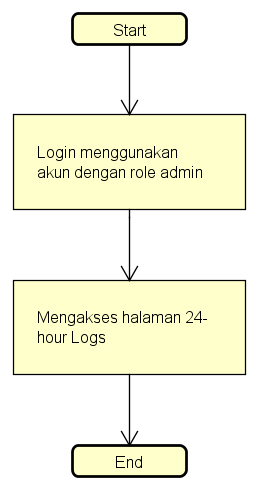
\includegraphics[width=1.0\textwidth]{logs}  
	\caption[\textit{Mockup} Halaman \textit{Logs}]{\textit{Mockup} Halaman \textit{Logs}} 
	\label{fig:logs} 
\end{figure}
Halaman ini terletak di paling bawah menu lainnya dan hanya dapat diakses oleh role admin.

\subsection{Membatasi Soal (Deskripsi \& PDF) Hanya Bisa Diakses saat \textit{Assignment} "\textit{Open}" dan Setelah Waktu Mulai}
Kebutuhan ini telah dibahas pada sub bab sebelumnya. Lihat sub bab \hyperref[subsec:membatasisoal]{3.1.8} untuk status dari kebutuhan ini.

\subsection{Mengumpulkan \textit{File} dengan Format TXT}
\label{subsec:filetxt}
Pengumpulan \textit{file} dengan format TXT dibutuhkan untuk \textit{Pre-test}. Perangkat lunak \textit{Sharif Judge} yang terkini hanya dapat menerima \textit{file} C, C++, Java, Python 2, Python 3, Zip, dan PDF. Para peserta yang ingin mengumupulkan jawaban \textit{Pre-test}, harus terlebih dahulu mengubah ekstensi \textit{file} menjadi Java atau mengompres \textit{file} ke dalam Zip. 

Pada skripsi ini, kebutuhan di atas diimplementasi. Solusi yang ditawarkan untuk kebutuhan di atas yaitu menambahkan \textit{file} dengan format TXT agar dapat dikumpul ke \textit{Sharif Judge}. \textit{Assignment} yang digunakan merupakan \textit{assignmnent} yang bersifat "\textit{Upload Only}". Dosen dapat menambahkan format TXT pada bagian "\textit{Allowed Language}" sehingga para peserta dapat mengumpulkan jawaban \textit{Pre-test} menggunakan \textit{file} dengan ekstensi TXT.

\subsection{Membatasi Soal (Deskripsi \& PDF) Hanya Bisa Diakses saat \textit{Assignment} "\textit{Open}" dan Setelah Waktu Mulai}
Kebutuhan ini telah dibahas pada sub bab sebelumnya. Lihat sub bab \hyperref[subsec:membatasisoal]{3.1.8} untuk status dari kebutuhan ini.

\subsection{Mengumpulkan \textit{File} dengan Format TXT}
Kebutuhan ini telah dibahas pada sub bab sebelumnya. Lihat sub bab \hyperref[subsec:filetxt]{3.1.12} untuk status dari kebutuhan ini.

\subsection{Perlu Ditambah Petunjuk Penamaan \textit{File} \textit{Input} dan \textit{Output}}
Dalam membuat sebuah assignment pada perangkat lunak \textit{Sharif Judge} terdapat \textit{file test case} yang harus disertakan. \textit{File test case} yang disertakan memiliki beberapa ketentuan. Beberapa ketentuan tersebut seperti struktur direktori dan penamaan dalam \textit{file test case}. 

Pada skripsi ini, kebutuhan di atas tidak diimplementasi. Pada halaman \textit{add assignment} telah disediakan \textit{link} menuju dokumentasi \textit{Sharif Judge} di \textit{GitHub} yang menjelaskan ketentuan dalam menyertakan \textit{file test case}. Ketentuan tersebut harus terpenuhi agar sebuah \textit{assignment} dapat berjalan dengan baik. Oleh sebab itu, kebutuhan ini tidak diimplementasi.

\subsection{Membatasi Soal (Deskripsi \& PDF) Hanya Bisa Diakses saat \textit{Assignment} "\textit{Open}" dan Setelah Waktu Mulai}
Kebutuhan ini telah dibahas pada sub bab sebelumnya. Lihat sub bab \hyperref[subsec:membatasisoal]{3.1.8} untuk status dari kebutuhan ini.

\subsection{Pendaftaran Peserta Disertai dengan \textit{Display Name}}
Pendaftaran peserta ke dalam \textit{Sharif Judge} terkini tidak disertai dengan \textit{Display Name}. Perangkat lunak \textit{Sharif Judge} membutuhkan empat buah parameter yang dipisah menggunakan spasi untuk mendaftarkan peserta. Parameter tersebut antara lain, \textit{username, \textit{email}, password} dan \textit{role}. Contoh penggunaannya seperti "\textit{i14085 i14085@unpar.ac.id random85 student}" yang artinya peserta didaftarkan menggunakan \textit{username} i14085, \textit{email} i14085@unpar.ac.id, \textit{password} random85 dan \textit{role} sebagai \textit{student}. Setiap peserta yang berhasil didaftarkan masih belum memiliki \textit{Display Name}. Para peserta harus memasukan \textit{Display Name} masing-masing secara manual. 

Pada skripsi ini, kebutuhan di atas diimplementasi. Solusi yang ditawarkan untuk memenuhi kebutuhan di atas yaitu menambahkan parameter \textit{Display Name} pada saat pendaftaran peserta. Pendaftaran peserta menggunakan lima buah paramater dan dipisah menggunakan tanda koma. Parameter tersebut antara lain,\textit{ username, email, display name, password,} dan \textit{role}. Contoh penggunaan parameter di atas seperti "\textit{i14085,i14085@unpar.ac.id,Budi Simon,random85,student}" yang artinya peserta didaftarkan menggunakan \textit{username} i14085, \textit{email} i14085@unpar.ac.id, \textit{display name} Budi Simon, \textit{password} random85 dan \textit{role} sebagai \textit{student}. Dengan pengimplementasian fitur ini, setiap peserta yang didaftarkan akan langsung memiliki Display Name masing-masing.

\subsection{Nama Pengguna \textit{Sharif Judge} Seharusnya Tidak Bisa Diubah}
\textit{Display Name} pada perangkat lunak \textit{Sharif Judge} berfungsi sebagai nama peserta. Selain itu, nama peserta akan muncul pada halaman \textit{Scoreboard} sebuah \textit{assignment} yang dapat dilihat oleh seluruh peserta. \textit{Sharif Judge} yang terkini mengijinkan para peserta untuk mengubah \textit{Display Name} pada halaman \textit{Profile}. Hal tersebut dapat dijadikan sebuah "mainan" dan tindakan kecurangan karena dapat memberikan \textit{hint} untuk peserta lain. Oleh karena itu, Ibu Joanna Helga menginginkan nama peserta yang terdaftar pada \textit{Sharif Judge} tidak dapat diubah. 

Pada skripsi ini, kebutuhan di atas diimplementasi. Solusi yang ditawarkan untuk memenuhi kebutuhan di atas yaitu menambahkan sebuah fitur dimana fitur tersebut dapat mengunci \textit{Display Name} peserta \textit{Sharif Judge}. Fitur ini diletakan pada halaman \textit{Settings} yang dapat diatur oleh \textit{admin}. Jika \textit{admin} mengaktifkan fitur tersebut, maka \textit{input text Display Name} pada halaman \textit{Profile} menjadi nonaktif sehingga para peserta tidak dapat mengubah \textit{Display Name}. Sebaliknya jika \textit{admin} menonaktifkan fitur tersebut, maka \textit{input text Display Name} pada halaman Profile akan kembali aktif.

\subsection{\textit{Sharif Judge} Diharapkan Memiliki Fungsi Dimana \textit{Assignment} Dapat Dikumpulkan Tanpa Adanya Batasan Waktu}
Pada masa Pra UTS dan Pra UAS biasanya para dosen akan memberikan \textit{assignment} sebagai bahan pembelajaran. Arsip-arsip soal ujian dan latihan tahun lalu akan dijadikan sebuah \textit{assignment} yang dapat dikerjakan oleh para peserta. \textit{Assignment} tersebut memiliki waktu pengumpulan yang cenderung lama. Ibu Joanna Helga menginginkan sebuah fitur dimana \textit{Sharif Judge} dapat mengatur \textit{assignment} tertentu menjadi tidak memiliki batasan waktu dan dapat dikumpulkan kapan saja. 

Pada skripsi ini, kebutuhan di atas diimplementasi. Solusi yang ditawarkan untuk memenuhi kebutuhan di atas yaitu membuat sebuah fitur tambahan pada \textit{assignment}. \textit{Assignment} yang mengaktifkan fitur ini tidak akan muncul pada kalendar yang terdapat di halaman \textit{Dashboard}. Fitur tersebut akan membuat batas waktu pengumpulan menjadi tanggal 18 Januari 2038. Tanggal 18 Januari 2038 diambil karena merupakan batas dari waktu \textit{UNIX}. Batas tersebut diperoleh karena setiap detik yang dilewati sejak tanggal 1 Januari 1970 disimpan menggunakan \textit{integer 32-bit}. Tanggal 18 Januari 2038 waktu UTC+7 merupakan batas maksimum dari \textit{integer 32-bit} tersebut. Masalah ini dikenal sebagai masalah "Year 2038 problem". 

\subsection{\textit{Sharif Judge} Diharapkan Memiliki \textit{Scoreboard Global} untuk Semua \textit{Assignment}}
\textit{Sharif Judge} terkini memiliki halaman \textit{Scoreboard} yang berfungsi menampilkan seluruh nilai akhir para peserta dari sebuah \textit{assignment}. Pada halaman \textit{Socreboard} juga menampilkan nilai dari setiap \textit{problem} yang ada pada sebuah \textit{assignment}. Nilai yang muncul pada halaman ini adalah nilai para peserta yang telah mengumpulkan jawabannya. Nilai yang muncul tersebut akan diurutkan mulai dari yang tertinggi hingga terendah. Ibu Joanna Helga menginginkan sebuah \textit{Scoreboard global} untuk semua \textit{assignment}. \textit{Scoreboard global} tersebut menampilkan total skor beserta detail skor setiap \textit{problem} yang telah dikerjakan para peserta diseluruh \textit{assignment} yang ada. 

Pada skripsi ini, kebutuhan di atas diimplementasi. Solusi yang ditawarkan untuk memenuhi kebutuhan di atas yaitu membuat halaman baru yang diberi nama \textit{Hall of Fame}. Halaman \textit{Hall of Fame} menampilkan berapa \textit{problem} yang telah dikerjakan oleh para peserta diseluruh \textit{assignment} yang ada. Nama peserta yang muncul pada halaman ini diurutkan sesuai dengan total skor dari seluruh \textit{assignment} yang telah dikerjakan oleh para peserta.

Berikut \textit{mockup} halaman \textit{Hall of Fame} yang diimplementasikan ke dalam perangkat lunak \textit{Sharif Judge}.
\begin{figure}[H]
	\centering  
	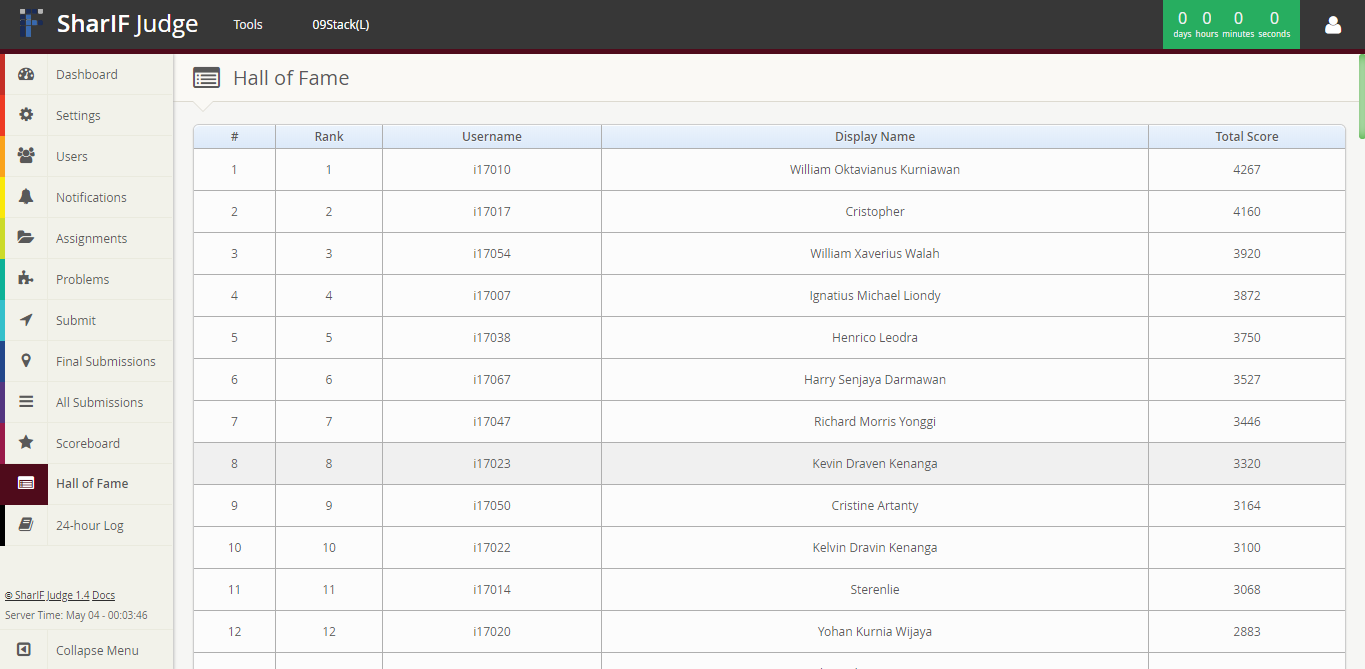
\includegraphics[width=1.0\textwidth]{hof}  
	\caption[\textit{Mockup} Halaman\textit{ Hall of Fame}]{\textit{Mockup} Halaman \textit{Hall of Fame}} 
	\label{fig:hof} 
\end{figure}
Halaman ini terletak di bawah menu halaman \textit{Scoreboard} dan dapat diakses oleh seluruh \textit{role}. Pada halaman Hall of Fame diberlakukan sistem rangking bedasarkan total skor yang diperoleh para peserta. Untuk melihat detail total skor yang dihasilkan dari setiap \textit{assignment}, para peserta dapat mengklik pada baris yang ada di tabel. Berikut contoh detail skor yang ditampilkan.
\begin{figure}[H]
	\centering  
	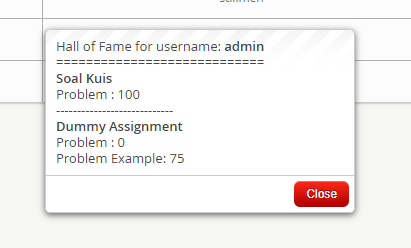
\includegraphics[scale=0.5]{hofdetail}  
	\caption[Detail Skor]{Detail Skor} 
	\label{fig:hofdetail} 
\end{figure}
Halaman kecil tersebut akan muncul dan berisikan nilai setiap \textit{problem} dari semua \textit{assignment} yang telah dikerjakan oleh peserta tertentu.

\subsection{Membatasi Soal (Deskripsi \& PDF) Hanya Bisa Diakses saat \textit{Assignment} "\textit{Open}" dan Setelah Waktu Mulai}
Kebutuhan ini telah dibahas pada sub bab sebelumnya. Lihat sub bab \hyperref[subsec:membatasisoal]{3.1.8} untuk status dari kebutuhan ini.

\subsection{Mengumpulkan \textit{File} dengan Format TXT}
Kebutuhan ini telah dibahas pada sub bab sebelumnya. Lihat sub bab \hyperref[subsec:filetxt]{3.1.12} untuk status dari kebutuhan ini.

\subsection{UI Masih Merepotkan}
Bapak Claudio Fransiscus mengeluhkan UI pada perangkat lunak \textit{Sharif Judge} merepotkan. Contohnya seperti pada saat peserta ingin memilih \textit{assignment}, para peserta harus masuk ke halaman \textit{assignment} dan memilih \textit{assignment} yang ingin dikerjakan. Contoh lainnya seperti skenario mengumpulkan jawaban, para peserta harus masuk ke halaman \textit{submit}, memilih \textit{problem} yang ingin dikumpulkan, memilih bahasa, memilih \textit{file} yang akan dikumpulkan dan \textit{submit}.

Pada skripsi ini, kebutuhan di atas tidak diimplementasi. Bapak Claudio Fransiscus masih kurang spesifik dalam menjelaskan kebutuhannya. Oleh karena kebutuhan tersebut kurang spesifik, maka pada skripsi ini kebutuhan di atas tidak diimplementasi.

\subsection{UI Ada yang Tidak Berguna}
Bapak Claudio Fransiscus mengeluhkan beberapa UI pada perangkat lunak \textit{Sharif Judge} tidak berguna. Pada \textit{side bar} \textit{Sharif Judge} terdapat beberapa menu halaman. Menurut Bapak Claudio Fransiscus, beberapa \textit{menu} tersebut tidak semuanya terpakai. \textit{Menu} yang sering digunakan hanya \textit{Assignments}, \textit{Submit}, Submission dan \textit{Scoreboard}.

Pada skripsi ini, kebutuhan di atas tidak diimplementasi. Claudio Fransiscus masih kurang spesifik dalam menjelaskan kebutuhannya. Oleh karena kebutuhan tersebut kurang spesifik, maka pada skripsi ini kebutuhan di atas tidak diimplementasi.

\subsection{\textit{Sharif Judge} Diharapkan Memiliki Fungsi \textit{Reminder}}
Setiap assignment pada perangkat lunak \textit{Sharif Judge} memiliki batas pengumpulan. Jika \textit{assignment} telah melewati batas pengumpulan maka para peserta tidak dapat mengumpulkan tugasnya. Banyak peserta sering kali lupa untuk mengerjakan \textit{assignment} dan pada akhirnya melewati batas pengumpulan. Bapak Claudio Fransiscus menginginkan perangkat lunak \textit{Sharif Judge} yang memiliki fitur \textit{reminder}. Fitur \textit{reminder} akan mengirimkan \textit{email} ke setiap peserta yang berisikan peringatan bahwa ada \textit{assignment} yang harus diselsaikan. 

Pada skripsi ini, kebutuhan di atas tidak diimplementasi. Kebutuhan di atas belum dapat diimplementasi karena masih belum ada sistem \textit{scheduler}. Selain itu, bobot pekerjaan diperkirakan akan membutuhkan waktu lebih dari 1 semester.

\subsection{Membatasi Soal (Deskripsi \& PDF) Hanya Bisa Diakses saat \textit{Assignment} "\textit{Open}" dan Setelah Waktu Mulai}
Kebutuhan ini telah dibahas pada sub bab sebelumnya. Lihat sub bab \hyperref[subsec:membatasisoal]{3.1.8} untuk status dari kebutuhan ini.

\subsection{Integrasi \textit{Login} ke \textit{Server RADIUS}}
\textit{RADIUS} (\textit{Remote Authentication Dial In User Service}) merupakan protokol jaringan klien dan \textit{server}. Klien mengirimkan informasi pengguna ke \textit{server RADIUS} yang ditunjuk dan akan bertindak berdasarkan respons yang dikembalikan. \textit{Server RADIUS} akan menerima permintaan koneksi pengguna, mengautentikasi pengguna dan kemudian mengembalikan informasi konfigurasi yang diperlukan agar klien dapat memberikan layanan kepada pengguna. \textit{Server RADIUS} dapat bertindak sebagai klien \textit{proxy} ke \textit{server RADIUS} lain atau \textit{server} autentikasi jenis lainnya \footnote{Cisco, "How Does RADIUS Work?" How Does RADIUS Work? - Cisco. \textit{https://www.cisco.com/c/en/us/support/docs/security-vpn/remote-authentication-dial-user-service-radius/12433-32.html} (diakses 22 Februari 2018)}. %footnote .
Lab FTIS UNPAR memiliki \textit{server RADIUS} yang dapat memverifikasi ID mahasiswa terhadap kata sandinya. \textit{Server RADIUS} juga berguna untuk autentikasi ID mahasiswa agar dapat menggunakan komputer di Lab FTIS UNPAR.

Pada skripsi ini, kebutuhan di atas diimplementasi. Solusi yang ditawarkan untuk memenuhi kebutuhan di atas yaitu mengintegrasikan \textit{login server RADIUS} pada perangkat lunak \textit{Sharif Judge}. Dengan pengimplementasian integrasi \textit{login RADIUS} pada \textit{Sharif Judge}, para peserta dapat \textit{login} ke \textit{Sharif Judge} menggunakan akun yang terdapat pada \textit{server RADIUS}. 

\subsection{Mengumpulkan \textit{File} dengan Format TXT}
Kebutuhan ini telah dibahas pada sub bab sebelumnya. Lihat sub bab \hyperref[subsec:filetxt]{3.1.12} untuk status dari kebutuhan ini.

\subsection{Mengumpulkan \textit{File} JAR (Java Multi Kelas)}
JAR (Java ARchive) adalah format \textit{file} platform-independen yang menggabungkan banyak \textit{file} menjadi satu. \textit{File-file} seperti kelas, gambar dan suara dapat digabungkan dalam \textit{file} JAR. Perangkat lunak \textit{Sharif Judge} yang terkini tidak mendukung pengumpulan \textit{file} dengan ekstensi JAR. \textit{Sharif Judge} hanya menerima beberapa tipe file yaitu C, C++, Java, Python 2, Python 3, Zip, dan PDF.

Pada skripsi ini, kebutuhan di atas tidak diimplementasi. %Solusi yang ditawarkan untuk kebutuhan di atas yaitu menambahkan file dengan format JAR agar dapat dikumpul ke \textit{Sharif Judge}. File dengan format JAR akan langsung dinilai oleh \textit{Sharif Judge} sehingga para peserta dapat melihat hasil dari jawaban masing-masing.

\subsection{Branding Teknik Informatika}
Branding Teknik Informatika dilakukan dengan cara mengubah logo dan ikon \textit{Sharif Judge} menjadi logo Teknik Informatika. Selain mengubah logo dan ikon, perubahan juga dilakukan terhadap nama perangkat lunak menjadi SharIF Judge dan link dokumentasi yang ada pada perangkat lunak \textit{Sharif Judge}. Hal di atas dapat dilakukan karena \textit{Sharif Judge} sendiri menggunakan lisensi GPL versi 3. GPL merupakan kepanjangan dari \textit{General Public License} yang memberikan beberapa kebebasan pada setiap penggunanya~\cite{brett:09:moss}.
Kebebasan tersebut antara lain:
	\begin{itemize}
		\item Kebebasan untuk menggunakan perangkat lunak dengan tujuan apapun \\
		\item Kebebasan untuk mengubah perangkat lunak sesuai dengan kebutuhan \\
		\item Kebebasan untuk membagikan perangkat lunak kepada teman dan kerabat \\
		\item Kebebasan untuk membagikan perubahan yang telah dilakukan
	\end{itemize}
Pada skripsi ini, kebutuhan di atas diimplementasi. Beberapa logo yang digunakan seperti:

\begin{figure}[H]
	\centering  
	
\includegraphics[scale=1]{logosmall}  
	\caption[Logo dan Ikon]{Logo dan Ikon} 
	\label{fig:logosmall} 
\end{figure} 

\begin{figure}[H]
	\centering  
	
\includegraphics[scale=1]{banner}  
	\caption[\textit{Banner Sharif Judge}]{\textit{Banner Sharif Judge}} 
	\label{fig:banner} 
\end{figure} 

Berikut beberapa tampilan \textit{Sharif Judge} yang baru.
\begin{figure}[H]
	\centering  
	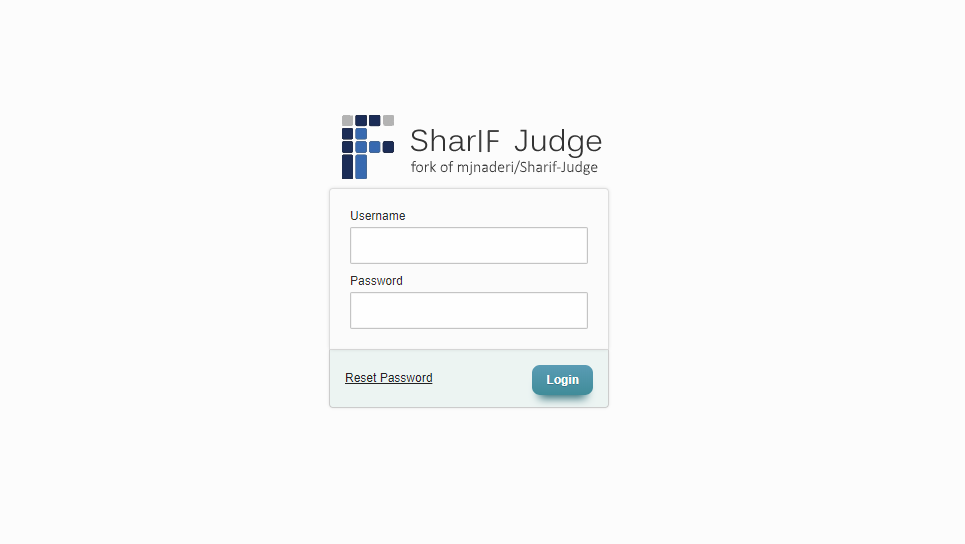
\includegraphics[scale=0.5]{login}  
	\caption[Halaman \textit{Login} \textit{Sharif Judge}]{Halaman \textit{Login} \textit{Sharif Judge}} 
	\label{fig:login} 
\end{figure}

\begin{figure}[H]
	\centering  
	
\includegraphics[scale=1]{ikon}  
	\caption[Ikon \textit{Sharif Judge} pada \textit{Title Bar}]{Ikon \textit{Sharif Judge} pada \textit{Title Bar}} 
	\label{fig:ikon} 
\end{figure} 

\begin{figure}[H]
	\centering  
	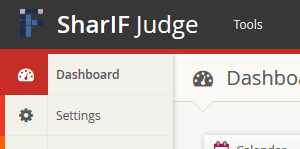
\includegraphics[scale=1]{logo}  
	\caption[Logo \textit{Sharif Judge} pada \textit{Top Bar}]{Logo \textit{Sharif Judge} pada \textit{Top Bar}} 
	\label{fig:logo} 
\end{figure} 

\subsection{Download Excel Tidak Berfungsi pada Halaman \textit{Submission}}
Perangkat lunak Sharif Judge yang terkini memiliki fitur yang dapat mengunduh excel pada halaman \textit{All Submission, Final Submission} dan \textit{Users}. Fitur ini berfungsi untuk memuat seluruh daftar \textit{All Submission, Final Submission} dan \textit{Users} ke dalam format excel. Agar fitur ini dapat berjalan dengan baik, \textit{Sharif Judge} menggunakan \textit{library} bantuan yaitu \textit{PHPExcel}. Versi \textit{PHP} yang digunakan oleh \textit{Sharif Judge} yang terkini tidak lagi mendukung \textit{library PHPExcel}. Hal tersebut menyebabkan fitur diatas menjadi tidak berfungsi. Dalam pengembangannya, \textit{PHPExcel} sudah tidak lagi digunakan. Para pengguna disarankan untuk migrasi ke \textit{library} penerusnya yaitu \textit{PhpSpreadsheet} atau alternatif lainnya \footnote{Adrien Crivelli, "PHPExcel - DEPRECATED" terakhir diubah 25 Desember 2017. \textit{https://github.com/PHPOffice/PHPExcel}}.

Pada skripsi ini, kebutuhan di atas diimplementasi. Solusi yang ditawarkan untuk kebutuhan di atas yaitu migrasi dari \textit{library} \textit{PHPExcel} ke \textit{PhpSpreadsheet} sehingga fitur mengunduh \textit{excel} pada halaman \textit{All Submission, Final Submission} dan \textit{Users} dapat berfungsi kembali.
\pagebreak

\section{Analisis Sistem Kini}

Seperti yang telah dibahas pada \hyperref[sec:sharifjudge]{Bab 2.2}, \textit{\textit{Sharif Judge}} menggunakan\textit{ framework Codeigniter}. \textit{Framework} ini menerapkan prinsip \textit{Model-View-Controller (M-V-C)}. \textit{Model-View-Controller} merupakan metode untuk membuat sebuah aplikasi dengan memisahkan data (\textit{Model}) dari tampilan (\textit{View}) dan cara memprosesnya (\textit{Controller}). Pada perangkat lunak \textit{Sharif Judge} \textit{model}, \textit{view} dan \textit{controller} terdapat pada folder \textit{Application} serta dipisahkan ke dalam masing-masing folder.  

\subsection{\textit{Model}}
Direktori model perangkat lunak \textit{Sharif Judge} terdapat pada \path{Sharif-Judge\application\models}. Di dalam folder \textit{models}, terdapat beberapa kelas model yang berisikan fungsi-fungsi untuk membantu pengguna mengambil, menyimpan, dan memperbarui informasi pada \textit{database}.

\subsubsection{\textit{Assignment\_Model.php}}
Pada \textit{file} \textit{Assignment\_Model.php} terdapat beberapa fungsi yaitu:
\begin{itemize}
	\item \textit{add\_assignment}: menambahkan \textit{assignment} baru ke dalam \textit{database} atau mengedit \textit{assignment} yang ada
	\item \textit{delete\_assignment}: menghapus \textit{assignment} 
	\item \textit{all\_assignments}: menampilkan semua daftar \textit{assignment} dan informasinya
	\item \textit{new\_assignment\_id}: mengembalikan nilai int terkecil yang dapat digunakan sebagai id untuk \textit{assignment} baru
	\item \textit{all\_problems}: mengembalikan \textit{array} yang berisi semua masalah dalam \textit{assignment} yang diberikan
	\item \textit{problem\_info}: mengembalikan baris \textit{database} untuk masalah tertentu
	\item \textit{assignment\_info}: mengembalikan baris \textit{database} untuk \textit{assignment} tertentu
	\item \textit{is\_participant}: mengecek apakah pengguna terdaftar sebagai peserta pada \textit{assignment} tertentu
	\item \textit{increase\_total\_submits}: meningkatkan jumlah total \textit{submit} sebanyak satu
	\item \textit{set\_moss\_time}: mengedit "\textit{Moss Update Time}" untuk \textit{assignment} tertentu
	\item \textit{get\_moss\_time}: mengembalikan "\textit{Moss Update Time}" untuk \textit{assignment} tertentu
	\item \textit{save\_problem\_description}: menambahkan atau Memperbarui deskripsi masalah
	\item \textit{\_update\_coefficients}: memperbarui koefisien yang terdapat pada \textit{assignment} tertentu. Fungsi ini dipanggil oleh fungsi \textit{add\_assignment}
\end{itemize}

\subsubsection{\textit{Notifications\_Model.php}}
Pada \textit{file} \textit{Notifications\_Model.php} terdapat beberapa fungsi yaitu:
\begin{itemize}
	\item \textit{get\_all\_notifications}: mengembalikan semua notifikasi
	\item \textit{get\_latest\_notifications}: mengembalikan 10 notifikasi terkini
	\item \textit{add\_notification}: menambahkan notifikasi baru
	\item \textit{update\_notification}: mengedit notifikasi tertentu
	\item \textit{delete\_notification}: menghapus notifikasi tertentu
	\item \textit{get\_notification}: menampilkan notifikasi tertentu
	\item \textit{have\_new\_notification}: mengecek apakah terdapat notifikasi setelah melewati waktu tertentu
\end{itemize}

\subsubsection{\textit{Queue\_Model.php}}
Pada \textit{file} \textit{Queue\_Model.php} terdapat beberapa fungsi yaitu:
\begin{itemize}
	\item \textit{in\_queue}: mengecek apakah sebuah submission telah berada dalam antrean
	\item \textit{get\_queue}: mengembalikan semua antrean \textit{submission}
	\item \textit{empty\_queue}: mengosongkan antrean
	\item \textit{add\_to\_queue}: memasukan \textit{submission} ke dalam antrean
	\item \textit{rejudge}: menambahkan \textit{submission} ke dalam antrean untuk di-\textit{rejudge}
	\item \textit{rejudge\_single}: menambahkan \textit{submission} tunggal ke dalam antrean untuk di-\textit{rejudge}
	\item \textit{get\_first\_item}: mengembalikan \textit{item} pertama dari antrean
	\item \textit{remove\_item}: menghapus \textit{item} tertentu dari antrean
	\item \textit{save\_judge\_result\_in\_db}: menyimpan hasil dari \textit{judge} ke dalam \textit{database}. Fungsi ini dipanggil oleh fungsi \textit{Queueprocess} di \textit{Controller}
\end{itemize}

\subsubsection{\textit{Scoreboard\_Model.php}}
Pada \textit{file} \textit{Scoreboard\_Model.php} terdapat beberapa fungsi yaitu:
\begin{itemize}
	\item \textit{\_generate\_scoreboard}: menghasilkan \textit{scoreboard} dari \textit{Final Submissions} untuk \textit{assignment} tertentu. Fungsi ini dipanggil oleh \textit{update\_scoreboard}
	\item \textit{update\_scoreboards}: mengupdate \textit{cache} \textit{scoreboard} dari semua \textit{assignment}. Fungsi ini dipanggil setiap kali pengguna menghapus atau semua \textit{assignment} pengguna dihapus.
	\item \textit{update\_scoreboard}: mengupdate \textit{cache scoreboard} dari semua \textit{assignment} dan menyimpan kode \textit{html scoreboard} ke dalam \textit{database}. Fungsi ini dipanggil setelah \textit{judging/rejudging} sebuah \textit{submission} dan ketika beberapa \textit{settings} diubah pada \textit{assignment} tertentu. \textit{Setting} tersebut terdiri dari \textit{Extra Time, Start Time, Finish Time, Coefficient's Rule} dan \textit{Enable/Disable Scoreboard}.
	\item \textit{get\_scoreboard}: mengembalikan \textit{cache} \textit{scoreboard} untuk \textit{assignment} tertentu sebagai teks \textit{html}
\end{itemize}

\subsubsection{\textit{Settings\_Model.php}}
Pada \textit{file} \textit{Settings\_Model.php} terdapat beberapa fungsi yaitu:
\begin{itemize}
	\item \textit{get\_setting}: mengembalikan pengaturan tertentu
	\item \textit{set\_setting}: mengupdate pengaturan tertentu
	\item \textit{get\_all\_settings}: menampilkan semua pengaturan
	\item \textit{set\_setting}: mengupdate seluruh pengaturan
\end{itemize}

\subsubsection{\textit{Submit\_Model.php}}
Pada \textit{file} Submit\_Model.php terdapat beberapa fungsi yaitu:
\begin{itemize}
	\item \textit{get\_submission}: mengembalikan baris tabel sebuah \textit{submission} tertentu 
	\item \textit{get\_final\_submissions}: mengembalikan baris tabel \textit{final submission} para peserta dari sebuah \textit{submission} tertentu
	\item \textit{get\_all\_submissions}: mengembalikan baris tabel seluruh \textit{submission}
	\item \textit{count\_final\_submissions}: mengembalikan jumlah total \textit{final submission} dari peserta tertentu
	\item \textit{count\_all\_submissions}: mengembalikan jumlah total \textit{submission} dari peserta tertentu
	\item \textit{set\_final\_submission}: menentukan \textit{submission} tertentu agar menjadi \textit{final submission}
	\item \textit{add\_upload\_only}: menambahkan hasil dari \textit{submit} "\textit{Upload only}" ke \textit{database}
\end{itemize}

\subsubsection{\textit{User.php}}
Pada \textit{file} \textit{User.php} terdapat beberapa fungsi yaitu:
\begin{itemize}
	\item \textit{select\_assignment}: menetapkan \textit{assignment} yang dipilih untuk username tertentu
	\item \textit{save\_widget\_positions}: mengupdate posisi dari \textit{dashboard widget} ke \textit{database}
	\item \textit{get\_widget\_positions}: mengembalikan posisi \textit{dashboard widget} dari \textit{database}
\end{itemize}

\subsubsection{\textit{User\_Model.php}}
Pada \textit{file} \textit{User\_Model.php} terdapat beberapa fungsi yaitu:
\begin{itemize}
	\item \textit{have\_user}: mengecek apakah pengguna dengan \textit{username} yang diinput terdapat di \textit{database}
	\item \textit{user\_id\_to\_username}: mengubah \textit{user id} menjadi \textit{username}
	\item \textit{username\_to\_user\_id}: mengubah \textit{username} menjadi \textit{user id}
	\item \textit{have\_email}: mengecek apakah pengguna dengan \textit{email} yang diberikan terdapat di \textit{database}
	\item \textit{add\_user}: menambahkan pengguna tunggal
	\item \textit{add\_users}: menambahkan beberapa pengguna
	\item \textit{delete\_user}: menghapus pengguna tertentu
	\item \textit{delete\_submissions}: menghapus semua \textit{submission} pengguna tertentu
	\item \textit{validate\_user}: mengecek apakah \textit{u}ser dan \textit{password} yang diinput cocok untuk keperluan \textit{login}
	\item \textit{selected\_assignment}: mengembalikan \textit{assignment} yang dipilih
	\item \textit{get\_names}: mengembalikan nama dari \textit{username} tertentu
	\item \textit{update\_profile}: memperbarui \textit{user profile} (\textit{Name, Email, Password, Role})
	\item \textit{send\_password\_reset\_mail}: Menghasilkan \textit{password reset key} dan mengirim \textit{email} berisi link untuk mereset \textit{password}
	\item \textit{passchange\_is\_valid}: mengecek apakah \textit{password reset key} sesuai
	\item \textit{reset\_password}: mereset \textit{password} untuk\textit{ password reset key} yang diberikan
	\item \textit{get\_all\_users}: menampilkan seluruh \textit{user} yang ada pada \textit{database}
	\item \textit{get\_user}: mengembalikan baris tabel \textit{user} dengan \textit{user id} tertentu
	\item \textit{update\_login\_time}: memperbaru \textit{First Login Time} dan \textit{Last Login Time username} tertentu	
\end{itemize}

\subsection{\textit{View}}
Pada perangkat lunak \textit{\textit{Sharif Judge}}, kelas view menggunakan \textit{framework} aplikasi yaitu \textit{Twig}. \textit{Twig} merupakan sebuah \textit{template engine modern} untuk \textit{PHP}. Beberapa kelebihannya adalah
\begin{itemize}
	\item Cepat: \textit{Twig} dapat mengcompile \textit{template} ke dalam kode \textit{HTML} dan dapat dioptimalkan. Dibandingkan dengan kode \textit{PHP} biasa, \textit{Twig} dapat menghasilkan kode \textit{PHP} menjadi seminimum mungkin.
	\item Aman: \textit{Twig} memiliki mode \textit{sandbox} untuk mengevaluasi kode template yang tidak tepercaya. Hal ini memungkinkan \textit{Twig} digunakan sebagai \textit{template language} untuk banyak aplikasi dimana pengguna dapat memodifikasi desain \textit{template} yang ada.
	\item Fleksibel: \textit{Twig} didukung oleh \textit{lexer} dan \textit{parser} yang fleksibel. Hal ini memungkinkan para pengembang untuk menentukan tag dan filter khusus~\cite{fabien:09:twig}.
\end{itemize}

Direktori \textit{view} perangkat lunak \textit{Sharif Judge} terdapat pada \path{Sharif-Judge\application\views}. Di dalam \textit{folder views}, terdapat beberapa \textit{folder} yang memisahkan kelas \textit{view} diantaranya adalah \textit{folder error}, \textit{pages} dan \textit{templates}. \textit{Folder error} berisikan tampilan ketika pengguna melakukan kesalahan seperti\textit{ 404 Page Not Found} atau \textit{Database Error}. \textit{Folder template} berisikan tampilan dasar penyusun \textit{Sharif Judge} seperti \textit{Top Bar, Side Bar} dan \textit{Header}. Folder pages berisikan tampilan utama \textit{\textit{Sharif Judge}}. Pada folder ini terdapat beberapa folder yaitu admin dan authtentication. \textit{Folder admin} berisikan tampilan yang hanya dapat dilihat oleh admin seperti tampilan \textit{Settings, User, Install, Add Assignemnt, Add Notification} dan lain-lain. \textit{Folder authentication} berisikan tampilan yang berhubungan dengan akses akun pengguna tampilan \textit{Login, Register} dan \textit{Reset Password}.

\subsubsection{\textit{dashboard.twig}}
\begin{figure}[H]
	\centering  
	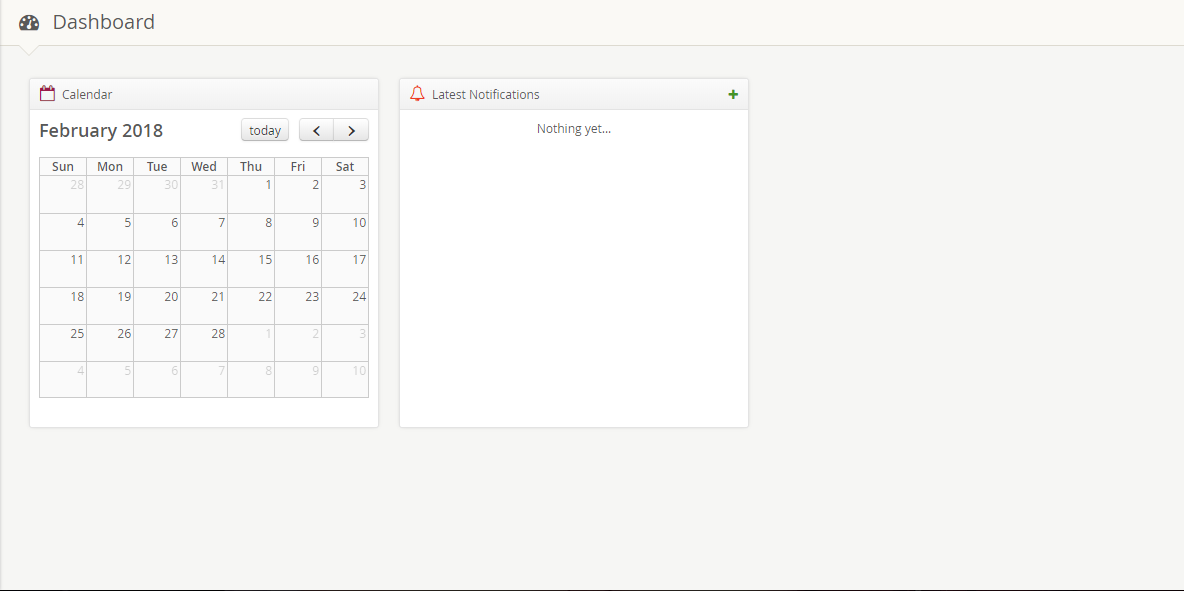
\includegraphics[scale=0.5]{dashboard}  
	\caption[\textit{Dashboard}]{\textit{Dashboard}} 
	\label{fig:dashboard} 
\end{figure} 
\textit{Dashboard} merupakan tampilan utama tepat setelah pengguna berhasil login pada perangkat lunak \textit{Sharif Judge}. Pada tampilan dashboard, terdapat kalendar dan tabel notifikasi. Kalendar akan menampilkan keterangan \textit{assignment} yang ada pada \textit{Sharif Judge}, sedangkan tabel notifikasi akan berisikan 10 pengumuman terbaru yang telah dibuat oleh admin.

\subsubsection{\textit{notifications.twig}}
\begin{figure}[H]
	\centering  
	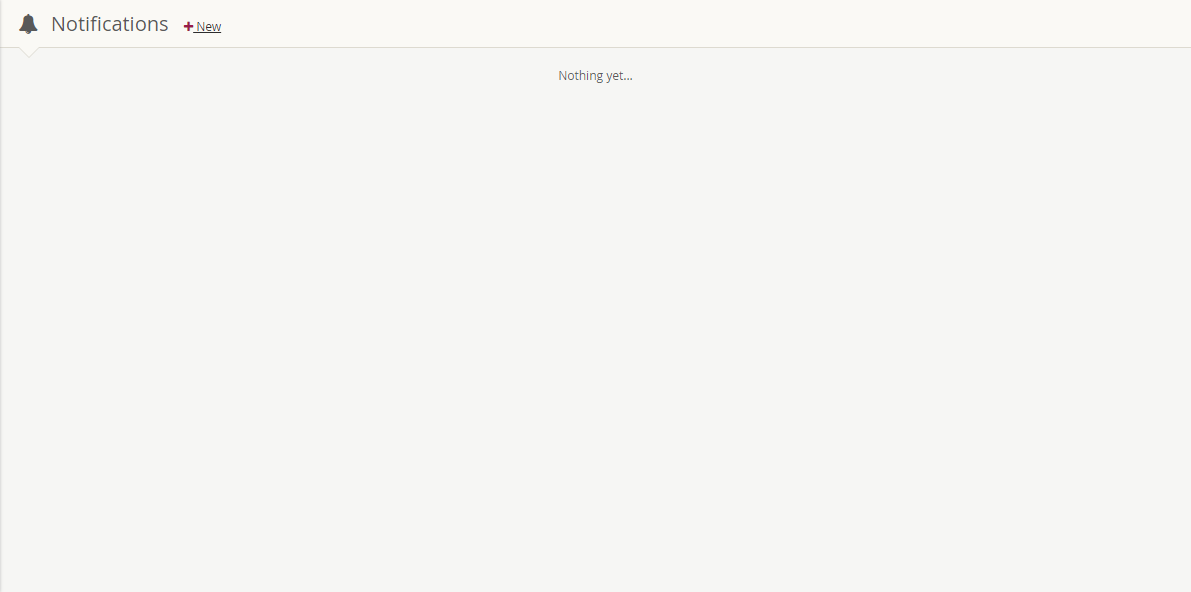
\includegraphics[scale=0.5]{notifications}  
	\caption[\textit{Notifications}]{\textit{Notifications}} 
	\label{fig:notifications} 
\end{figure} 
Halaman notifikasi berisikan seluruh notifikasi yang telah dibuat oleh admin. Jika admin yang memasuki halaman tersebut, maka terdapat pilihan "\textit{New}" dimana admin dapat menambahkan pengumuman baru untuk para pengguna \textit{Sharif Judge}. Pengumuman tersebut akan munucl pada tabel notifikasi di \textit{dashboard}.

\subsubsection{\textit{assignments.twig}}
\begin{figure}[H]
	\centering  
	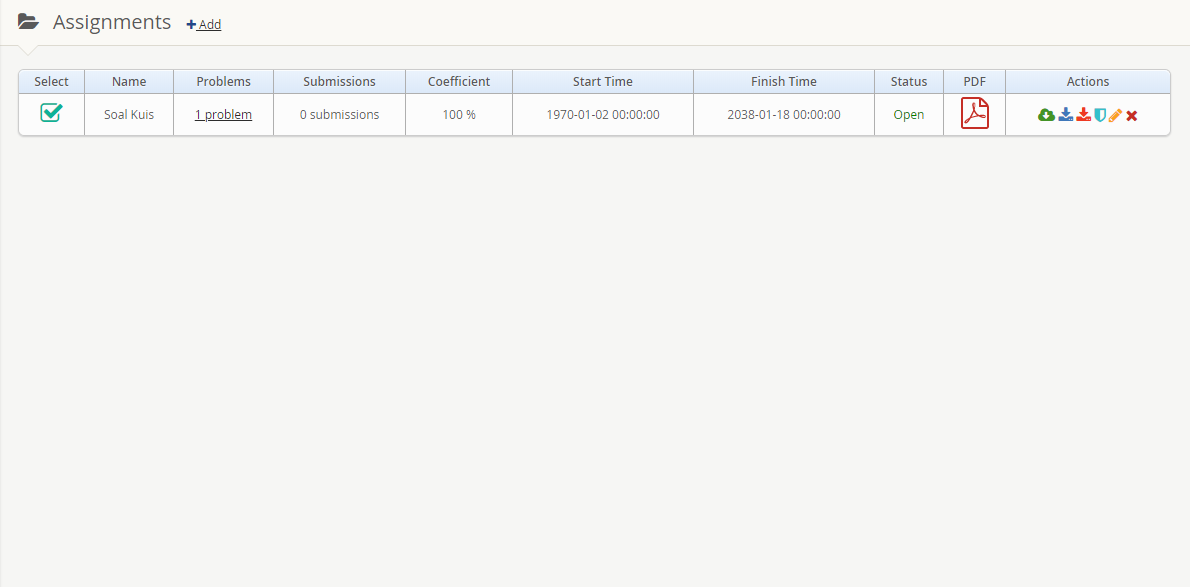
\includegraphics[scale=0.5]{assignments}  
	\caption[\textit{Assignments}]{\textit{Assignments}} 
	\label{fig:assignments} 
\end{figure} 
Halaman \textit{assignments} berisikan seluruh \textit{assignment} yang ada pada \textit{Sharif Judge}. Pada halaman ini, pengguna dapat memilih \textit{assignment} mana yang akan dikerjakan. Jika admin yang memasuki halaman tersebut, maka terdapat beberapa pilihan tambahan. Beberapa pilihan tambahan seperti fungsi "\textit{Add}" akan mengarahkan admin ke halaman baru untuk menambah \textit{assignment} dan beberapa fungsi lain untuk mengedit, menghapus atau mengunduh \textit{assignment} yang sudah ada.

\subsubsection{\textit{problems.twig}}
\begin{figure}[H]
	\centering  
	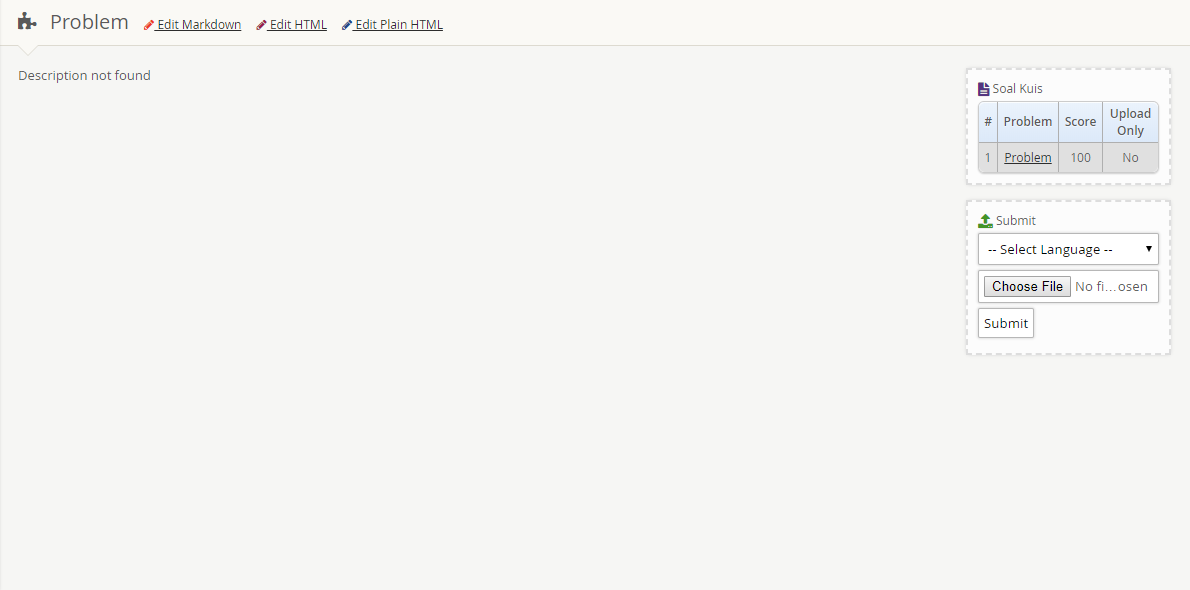
\includegraphics[scale=0.5]{problems}  
	\caption[\textit{Problems}]{\textit{Problems}} 
	\label{fig:problems} 
\end{figure} 
Halaman \textit{problems} berisikan masalah-masalah yang ada pada suatu \textit{assignment}. Pada halaman ini, pengguna dapat melihat diskripsi pada masing-masing masalah. Selain melihat diskripsi masalah, para pengguna juga dapat mengumpulkan jawaban dari setiap masalah tersebut.

\subsubsection{\textit{submit.twig}}
\begin{figure}[H]
	\centering  
	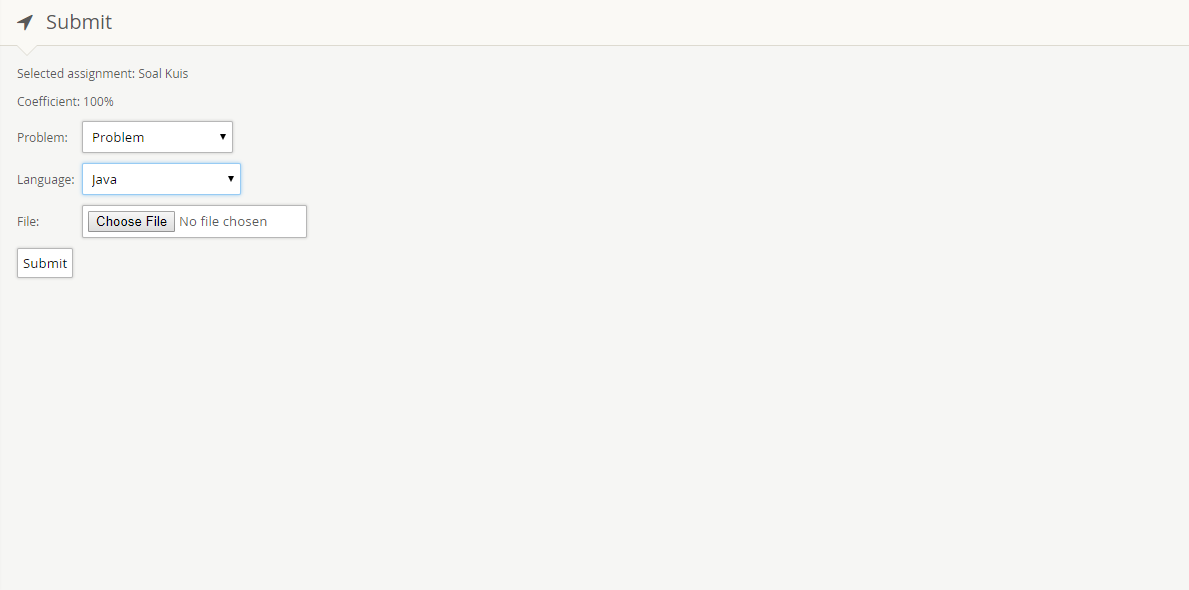
\includegraphics[scale=0.5]{submit}  
	\caption[\textit{Submit}]{\textit{Submit}} 
	\label{fig:submit} 
\end{figure} 
Halaman \textit{submit} berfungsi untuk mengumpulkan jawaban dari \textit{assignment} yang telah dipilih pengguna sebelumnya. Pengguna dapat memilih masalah telah diselsaikan lalu memilih bahasa yang digunakan dan memilih \textit{file} jawaban yang akan dikumpulkan. Setelah mengumpulkan jawaban, pengguna akan diarahkan ke halaman \textit{All Submission} untuk melihat hasil dari jawaban yang telah dikumpulkan sebelumnya.

\subsubsection{\textit{profile.twig}}
\begin{figure}[H]
	\centering  
	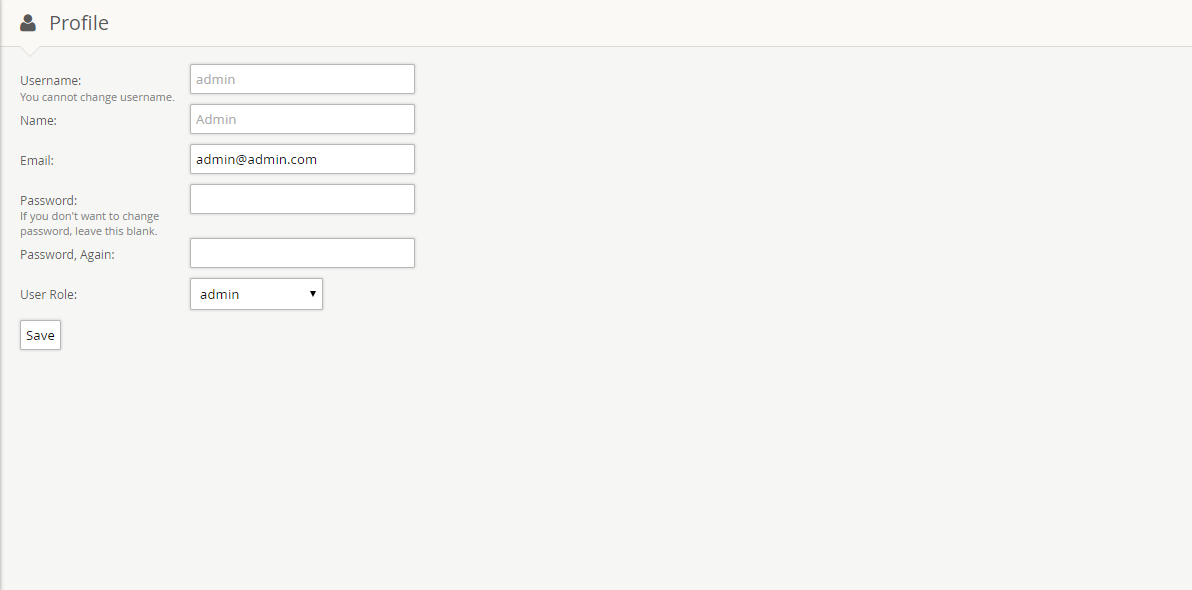
\includegraphics[scale=0.5]{profile}  
	\caption[\textit{Profile}]{\textit{Profile}} 
	\label{fig:profile} 
\end{figure} 
Halaman \textit{profile} berisikan keterangan akun pengguna \textit{Sharif Judge}. Pada halaman ini, pengguna dapat mengubah nama, \textit{email} dan \textit{password}. Jika admin yang memasuki halaman ini, maka terdapat tambahan pilihan yaitu \textit{user role}. Admin dapat mengubah user role menjadi \textit{head\_instructor, instructor} dan \textit{student}.

\subsubsection{\textit{scoreboard.twig}}
\begin{figure}[H]
	\centering  
	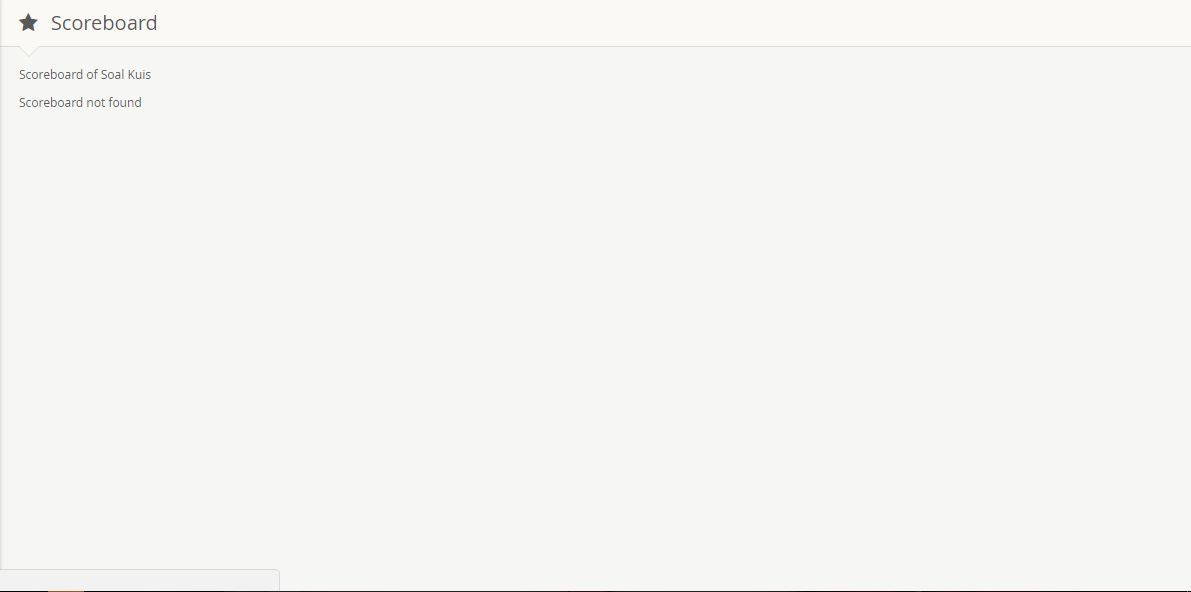
\includegraphics[scale=0.5]{scoreboard}  
	\caption[\textit{Scoreboard}]{\textit{Scoreboard}} 
	\label{fig:scoreboard} 
\end{figure} 
Halaman \textit{scoreboard} berisikan nilai seluruh pengguna \textit{Sharif Judge} pada \textit{assignment} tertentu. Nama pengguna yang muncul akan terurut secara menurun bedasarkan nilai \textit{assignment} pengguna. Admin dapat menonaktifkan \textit{scoreboard} dengan cara menghilangkan \textit{checklist} "\textit{Scoreboard}" pada halaman \textit{Add Assignment}.

\subsubsection{\textit{submission.twig}}
\begin{figure}[H]
	\centering  
	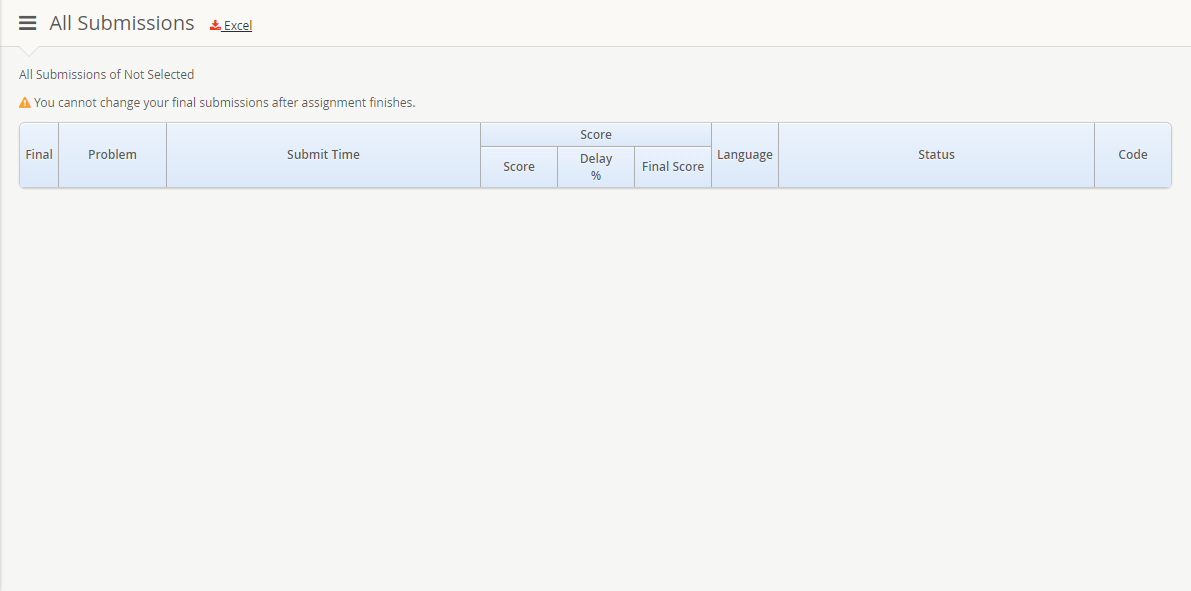
\includegraphics[scale=0.5]{allsubmission}  
	\caption[\textit{All Submission}]{\textit{All Submission}} 
	\label{fig:allsubmission} 
\end{figure} 

\begin{figure}[H]
	\centering  
	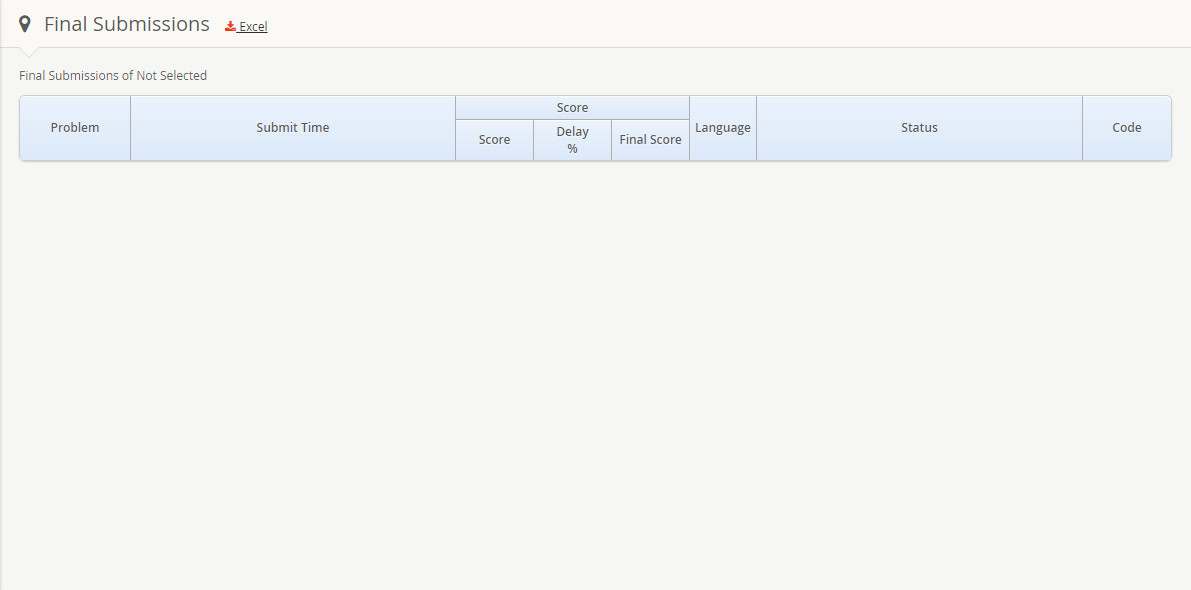
\includegraphics[scale=0.5]{finalsubmission}  
	\caption[\textit{Final Submission}]{\textit{Final Submission}} 
	\label{fig:finalsubmission} 
\end{figure} 

\textit{File} \textit{submission.twig} terbagi menjadi dua halaman yaitu \textit{All Submission} dan \textit{Final Submission}. Pada halaman \textit{All Submission}, pengguna dapat melihat seluruh jawaban yang telah dikumpulkan. Pengguna juga dapat memilih salah satu jawaban dari suatu masalah yang akan dijadikan jawaban akhir. Pada halaman \textit{Final Submission}, pengguna dapat melihat seluruh jawaban akhir yang telah dipilih sebelumnya di halaman \textit{All Submission}.

\subsubsection{\textit{settings.twig}}
\begin{figure}[H]
	\centering  
	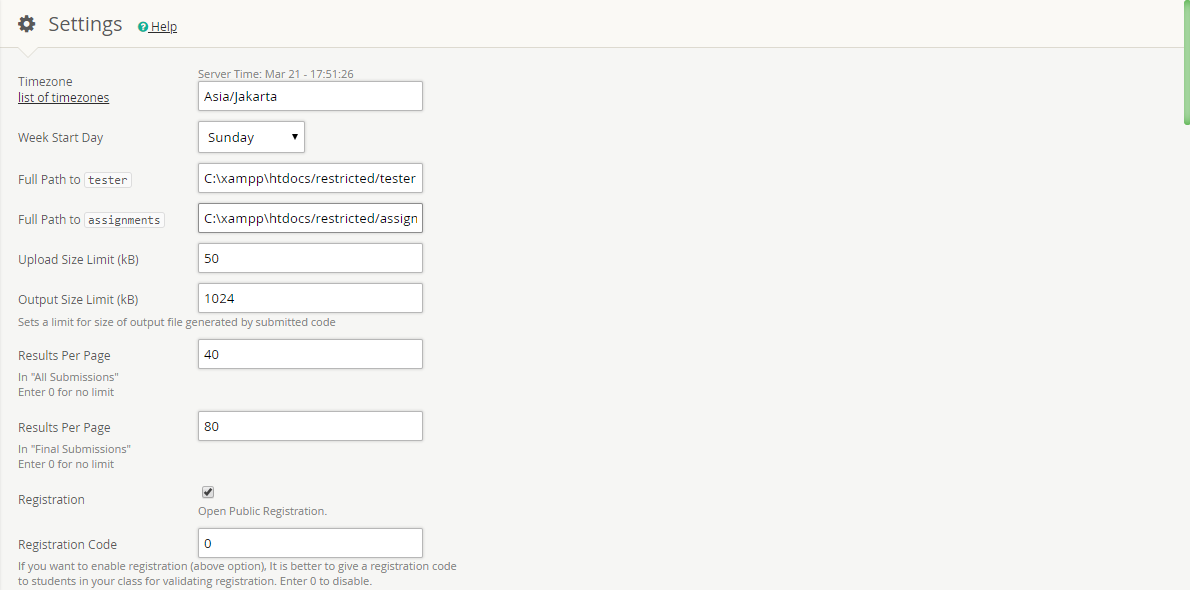
\includegraphics[scale=0.5]{settings}  
	\caption[\textit{Settings}]{\textit{Settings}} 
	\label{fig:settings} 
\end{figure} 
Halaman \textit{settings} berisikan pengaturan yang ada pada \textit{Sharif Judge}. Beberapa pengaturannya yaitu pengaturan \textit{timezone}, direktori \textit{assignments}, direktori \textit{tester}, \textit{email}, \textit{sandboxing}, \textit{shield} dan lain-lain.

\subsubsection{\textit{user.twig}}
\begin{figure}[H]
	\centering  
	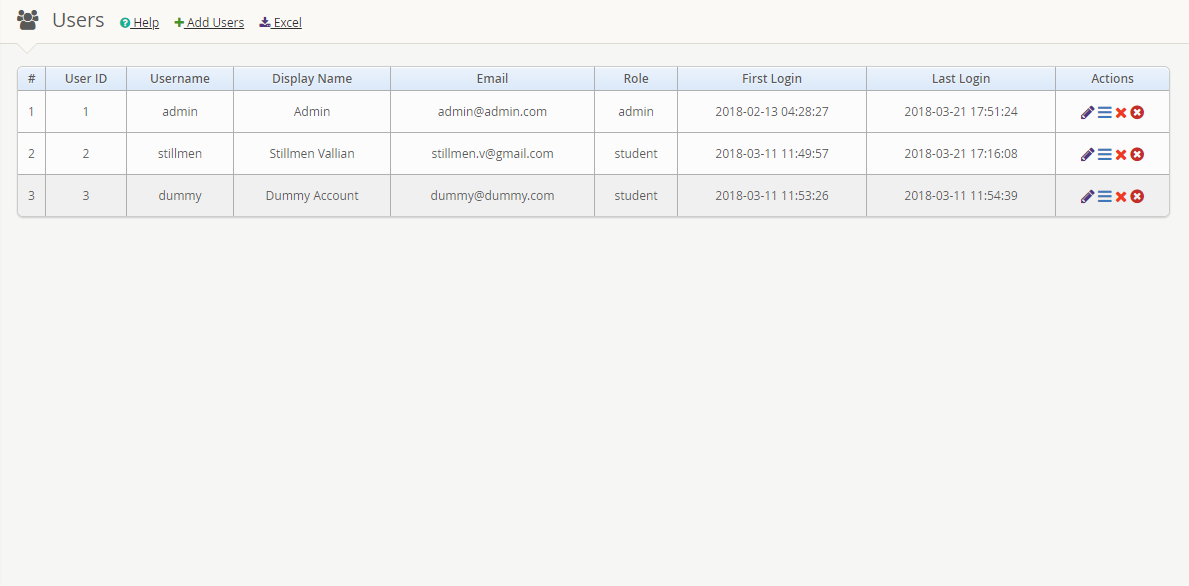
\includegraphics[scale=0.5]{user}  
	\caption[\textit{User}]{\textit{User}} 
	\label{fig:user} 
\end{figure} 
Halaman \textit{user} berisikan list pengguna yang terdaftar pada \textit{Sharif Judge}. Pada halaman ini, admin dapat melakukan beberapa aksi seperti menambah pengguna, menghapus pengguna, melihat hasil jawaban pengguna, menghapus jawaban pengguna dan mengubah data diri pengguna. 

\subsubsection{\textit{add\_user.twig}}
\begin{figure}[H]
	\centering  
	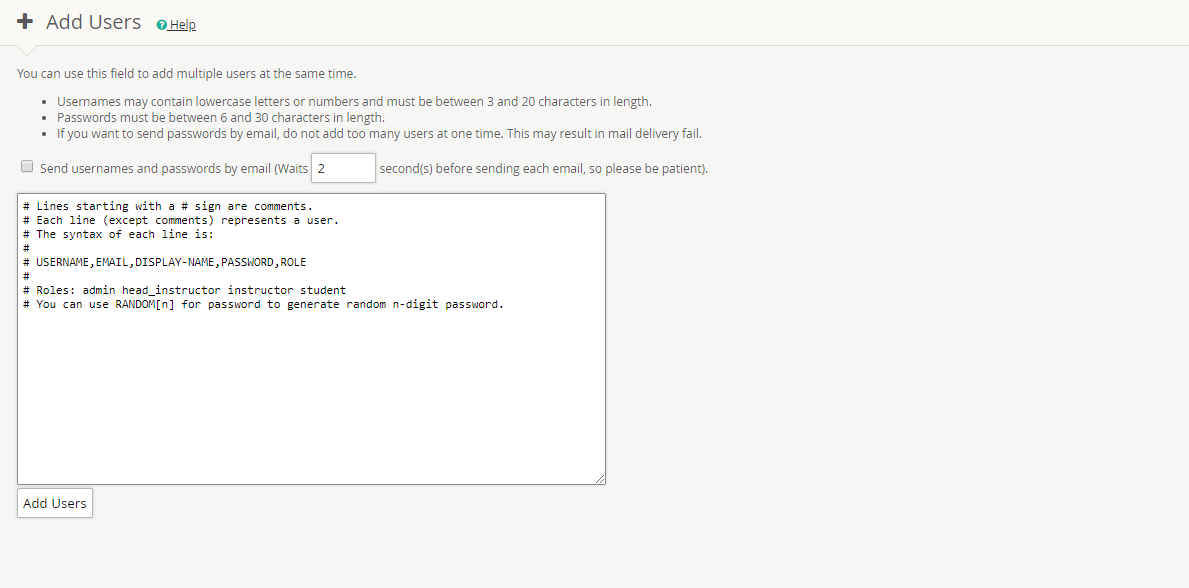
\includegraphics[scale=0.5]{adduser}  
	\caption[\textit{Add User}]{\textit{Add User}} 
	\label{fig:adduser} 
\end{figure} 
Halaman \textit{add user} berfungsi untuk menambah peserta pada \textit{Sharif Judge}. Pada halaman ini, admin dapat memasukan informasi pengguna yang ingin didaftarkan pada \textit{Sharif Judge}. Informasi tersebut berupa \textit{username}, \textit{email}, \textit{password} dan \textit{role}.

\subsubsection{\textit{add\_notification.twig}}
\begin{figure}[H]
	\centering  
	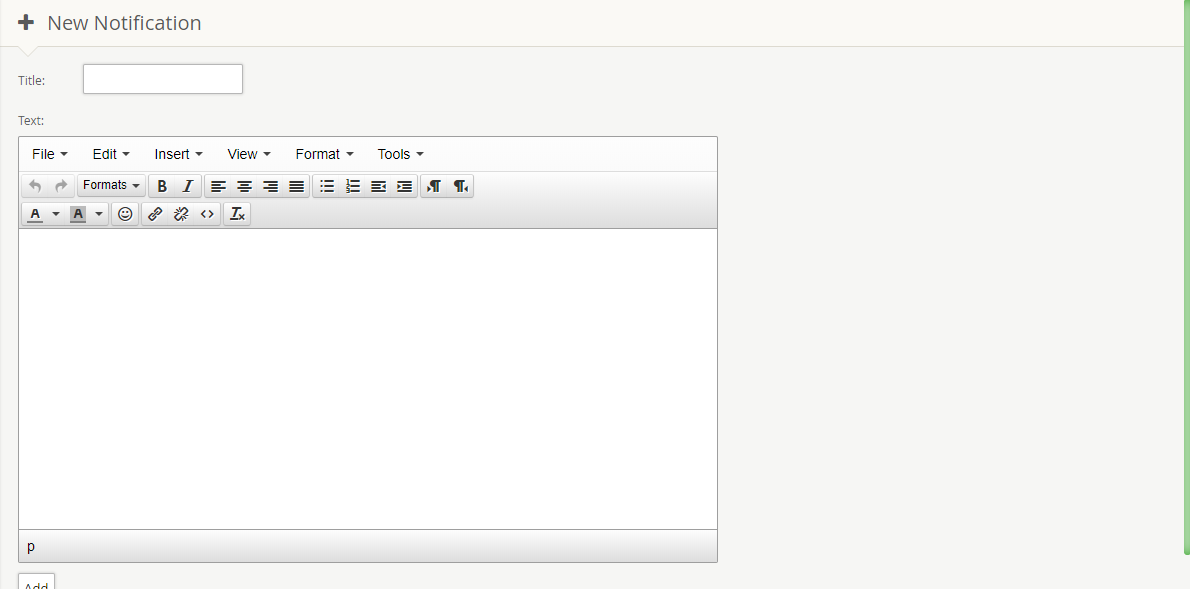
\includegraphics[scale=0.5]{addnotification}  
	\caption[\textit{Add Notification}]{\textit{Add Notification}} 
	\label{fig:addnotification} 
\end{figure} 
Halaman \textit{add notification} berfungsi untuk menambah pengumuman pada \textit{Sharif Judge}. Pada halaman ini, terdapat beberapa \textit{form} seperti judul pengumuman dan isi dari pengumuman tersebut.  

\subsubsection{\textit{add\_assignment.twig}}
\begin{figure}[H]
	\centering  
	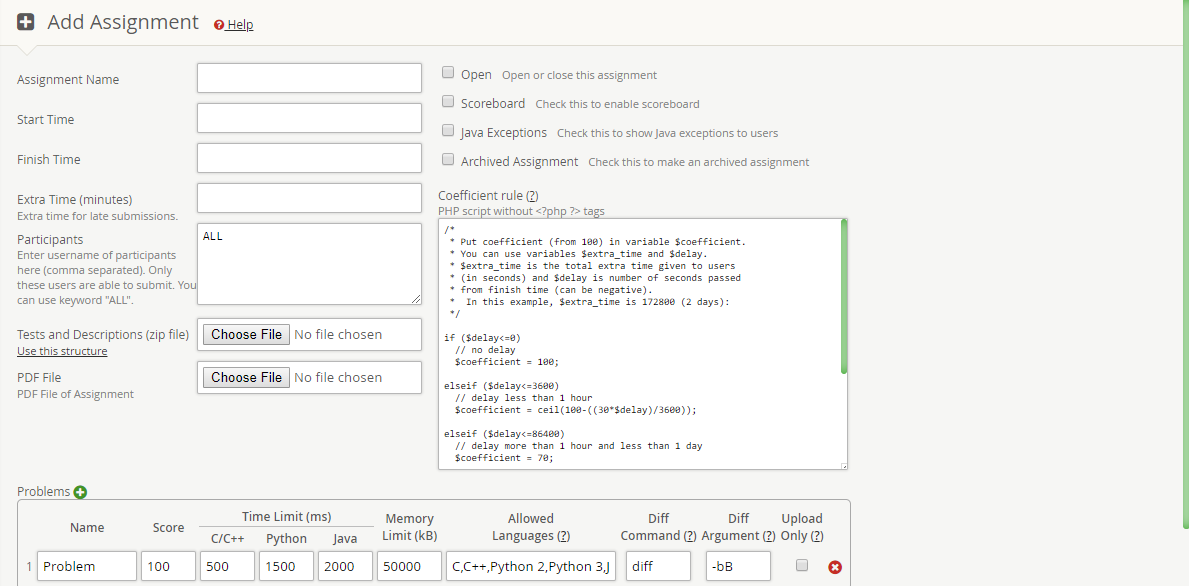
\includegraphics[scale=0.5]{addassignment}  
	\caption[\textit{Add Assignment}]{\textit{Add Assignment}} 
	\label{fig:addassignment} 
\end{figure} 
Halaman \textit{add assignment} berfungsi untuk menambah \textit{assignment} pada \textit{Sharif Judge}. Pada halaman ini, \textit{admin} dan \textit{head instructor} dapat mengatur beberapa pengaturan \textit{assignment} tersebut. Beberapa pengaturan seperti nama, waktu mulai, waktu akhir, \textit{scoreboard} dan lain-lain. \textit{Admin} juga dapat mengunggah diskripsi serta \textit{file} PDF untuk \textit{assignment} tersebut.

\subsubsection{\textit{rejudge.twig}}
\begin{figure}[H]
	\centering  
	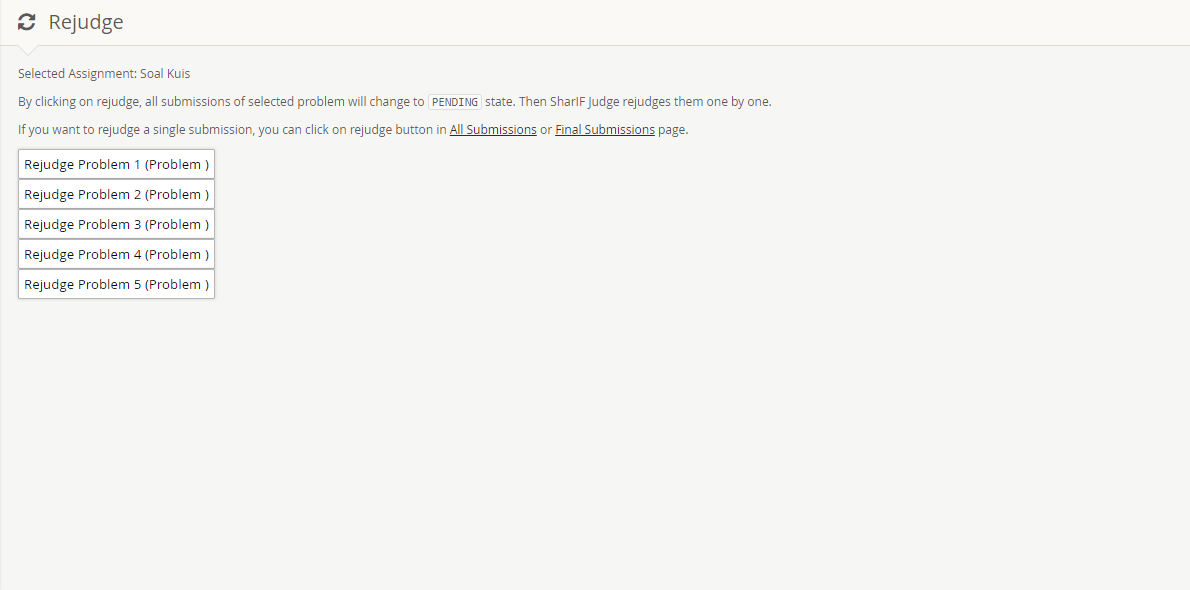
\includegraphics[scale=0.5]{rejudge}  
	\caption[\textit{Rejudge}]{\textit{Rejudge}} 
	\label{fig:rejudge} 
\end{figure} 
Halaman \textit{rejudge} berfungsi untuk menilai ulang hasil pekerjaan seluruh peserta \textit{Sharif Judge}. Pada halaman ini, \textit{admin} dan \textit{head instructor} dapat menilai ulang setiap masalah pada \textit{assignment} yang dipilih.

\subsubsection{\textit{login.twig}}
\begin{figure}[H]
	\centering  
	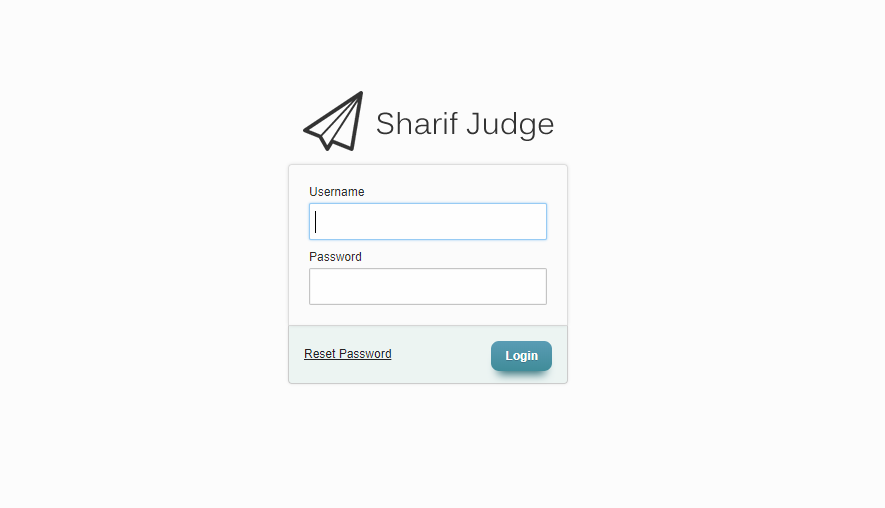
\includegraphics[scale=0.5]{loginold}  
	\caption[\textit{Login}]{\textit{login}} 
	\label{fig:oldlogin} 
\end{figure} 
Halaman login merupakan halaman pertama yang tampil ketika pengguna membuka \textit{Sharif Judge}. Untuk dapat menggunakan \textit{Sharif Judge}, para pengguna harus memasukan kombinasi \textit{username} dan \textit{password} yang tepat. Jika pengguna berhasil \textit{login}, maka akan diarahkan ke halaman \textit{dashboard}. Jika pengguna gagal \textit{login}, maka akan muncul pesan kesalahan "\textit{Incorrect username or password}" .

\subsubsection{\textit{register.twig}}
\begin{figure}[H]
	\centering  
	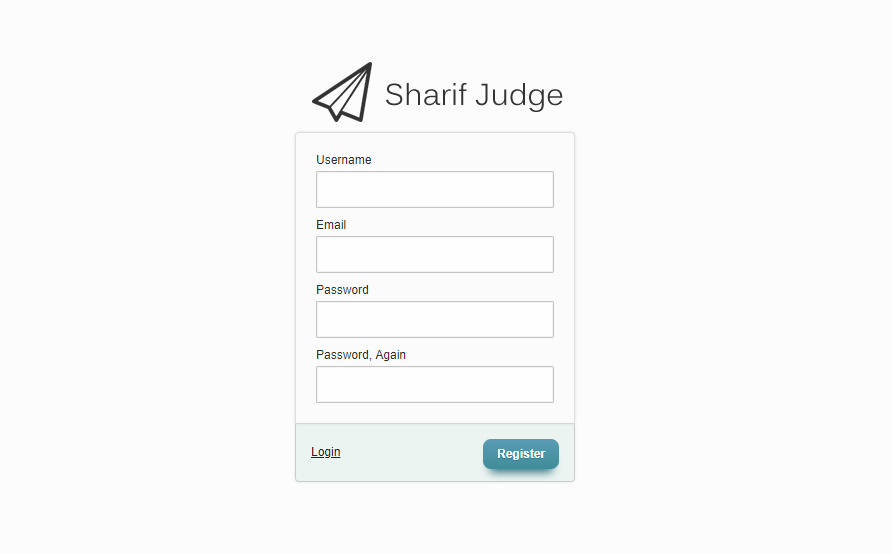
\includegraphics[scale=0.5]{register}  
	\caption[\textit{Register}]{\textit{Register}} 
	\label{fig:register} 
\end{figure} 
Halaman \textit{register} berfungsi untuk mendaftar sebagai peserta \textit{Sharif Judge}. Umumnya halaman ini tidak tersedia karena pengguna \textit{Sharif Judge} telah ditentukan sebelumnya oleh \textit{admin} dan \textit{head instructor}. Halaman ini akan muncul jika \textit{admin} mengaktifkan fitur \textit{Open Public Registration} pada halaman \textit{Settings}.

\subsubsection{\textit{lost.twig}}
\begin{figure}[H]
	\centering  
	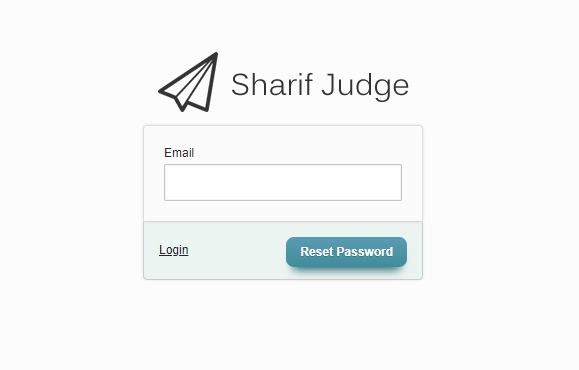
\includegraphics[scale=0.5]{lost}  
	\caption[\textit{Lost}]{\textit{Lost}} 
	\label{fig:lost} 
\end{figure} 
Halaman \textit{lost} berfungsi untuk para peserta yang lupa kombinasi \textit{username} dan \textit{password}. Peserta harus memasukan \textit{email} yang didaftarkan pada \textit{Sharif Judge}. \textit{Sharif Judge} akan mengirimkan \textit{link} untuk mereset \textit{password} ke \textit{email} yang telah dimasukan sebelumnya.

\subsection{\textit{Controller}}
Direktori \textit{controller} perangkat lunak \textit{Sharif Judge} terdapat pada \path{Sharif-Judge\application\controllers}.Di dalam \textit{folder controllers}, terdapat beberapa kelas \textit{controller} yang berisikan fungsi-fungsi sebagai perantara antara \textit{model, view}, dan \textit{resource} lainnya yang dibutuhkan untuk memproses \textit{HTTP request}.

\subsubsection{\textit{Assignments.php}}
Pada \textit{file} \textit{Assignments.php} terdapat beberapa fungsi yaitu:
\begin{itemize}
	\item \textit{index}: mempersiapkan data yang dibutuhkan untuk halaman \textit{assignments.twig}. Data yang dipersiapkan, diambil menggunakan fungsi-fungsi yang terdapat pada \textit{Assignment\_model.php}
	\item \textit{select}: memilih \textit{assignment} yang ada pada \textit{Sharif Judge}
	\item \textit{pdf}: mengunduh \textit{file} pdf atau deskripsi masalah pada \textit{assignment} tertentu
	\item \textit{downloadtestsdesc}: mengompres dan mengunduh test data dan deskripsi \textit{assignment} tertentu
	\item \textit{download\_submissions}: mengompres dan mengunduh jawaban akhir para peserta pada \textit{assignment} tertentu
	\item \textit{delete}: menghapus sebuah \textit{assignment}
	\item \textit{add}: mengambil input dari user untuk menambah atau mengubah \textit{assignment}
	\item \textit{\_add}: menambah atau mengubah \textit{assignment}
\end{itemize}

\subsubsection{\textit{Dashboard.php}}
Pada \textit{file} \textit{Dashboard.php} terdapat beberapa fungsi yaitu:
\begin{itemize}
	\item \textit{index}: mempersiapkan data yang dibutuhkan untuk halaman \textit{dashboard.twig}. Data yang dipersiapkan, diambil menggunakan beberapa fungsi yang terdapat pada \textit{Assignment\_model.php}, \textit{Settings\_model.php} dan \textit{Notification\_model.php}
	\item \textit{widget\_positions}: menyimpan posisi \textit{widget} pada \textit{Dashboard} pengguna
\end{itemize}

\subsubsection{\textit{Install.php}}
Pada \textit{file} \textit{Install.php} terdapat beberapa fungsi yaitu:
\begin{itemize}
	\item \textit{index}: fungsi ini membuat table-table yang dibutuhkan oleh \textit{Sharif Judge} ke \textit{database} yang telah ditentukan
\end{itemize}

\subsubsection{\textit{Login.php}}
Pada \textit{file} \textit{Login.php} terdapat beberapa fungsi yaitu:
\begin{itemize}
	\item \textit{\_registration\_code}: memeriksa apakah kode pendaftaran yang dimasukkan sudah benar atau tidak
	\item \textit{index}: memvalidasi kombinasi antara \textit{username} dan \textit{password} yang telah dimasukan pengguna
	\item \textit{register}: mempersiapakan \textit{form} registrasi dan memproses tampilan pada \textit{register.twig}
	\item \textit{logout}: keluar dari \textit{Sharif Judge} dan mengalihkan pengguna ke halanan \textit{login}
	\item \textit{lost}: mempersiapakan \textit{form} lupa \textit{password} dan memproses tampilan pada \textit{lost.twig}
\end{itemize}

\subsubsection{\textit{Notification.php}}
Pada \textit{file} \textit{Notification.php} terdapat beberapa fungsi yaitu:
\begin{itemize}
	\item \textit{index}: mempersiapkan data yang dibutuhkan untuk halaman \textit{notification.twig}. Data yang dipersiapkan, diambil menggunakan beberapa fungsi yang terdapat pada \textit{Assignment\_model.php} dan \textit{Notification\_model.php}
	\item \textit{add}: menambah pengumuman pada \textit{Sharif Judge}
	\item \textit{edit}: mengubah pengumuman yang ada pada \textit{Sharif Judge}
	\item \textit{delete}: menghapus pengumuman yang ada pada \textit{Sharif Judge}
\end{itemize}

\subsubsection{\textit{Problems.php}}
Pada \textit{file} \textit{Problems.php} terdapat beberapa fungsi yaitu:
\begin{itemize}
	\item \textit{index}: menampilkan deskripsi \textit{problem} yang diberikan
	\item \textit{edit}: mengubah diskripsi \textit{problem} yang ada pada \textit{Sharif Judge}
\end{itemize}

\subsubsection{\textit{Profile.php}}
Pada \textit{file} \textit{Profile.php} terdapat beberapa fungsi yaitu:
\begin{itemize}
	\item \textit{index}: mempersiapkan \textit{form profile} yang berfungsi untuk mengubah informasi dari pengguna \textit{Sharif Judge}
	\item \textit{\_password\_check}: mengecek apakah \textit{password} yang dibuat oleh pengguna \textit{Sharif Judge} memenuhi syarat. Syarat \textit{password} tersebut yaitu minimal terdiri dari 6 karakter.
	\item \textit{\_password\_again\_check}: mengecek apakah '\textit{password again}' yang dimasukan sama dengan password yang telah dimasukan sebelumnya
	\item \textit{\_email\_check}: mengecek apakah \textit{email} yang dimasukan pengguna telah digunakan pengguna lain
	\item \textit{\_role\_check}: memvalidasi \textit{user role}
\end{itemize}

\subsubsection{\textit{Queueprocess.php}}
Pada \textit{file} \textit{Queueprocess.php} terdapat beberapa fungsi yaitu:
\begin{itemize}
	\item \textit{run}: fungsi utama untuk memproses antrean (\textit{queue}) dimana fungsi ini menjudge antrean satu demi satu
\end{itemize}

\subsubsection{\textit{Rejudge.php}}
Pada \textit{file} \textit{Rejudge.php} terdapat beberapa fungsi yaitu:
\begin{itemize}
	\item \textit{index}: mempersiapkan data yang dibutuhkan untuk halaman \textit{rejudge.twig}. Data yang dipersiapkan, diambil menggunakan beberapa fungsi yang terdapat pada \textit{Assignment\_model.php}
	\item \textit{rejudge\_single}: menilai ulang jawaban peserta pada satu masalalah tertentu
\end{itemize}

\subsubsection{\textit{Scoreboard.php}}
Pada \textit{file} \textit{Scoreboard.php} terdapat beberapa fungsi yaitu:
\begin{itemize}
	\item \textit{index}: mempersiapkan data yang dibutuhkan untuk halaman \textit{scoreboard.twig}. Data yang dipersiapkan, diambil menggunakan beberapa fungsi yang terdapat pada \textit{Assignment\_model.php} dan \textit{Scoreboard\_model.php}
\end{itemize}

\subsubsection{\textit{Server\_time.php}}
Pada \textit{file} \textit{Server\_time.php} terdapat beberapa fungsi yaitu:
\begin{itemize}
	\item \textit{index}: menampilkan waktu server yang berfungsi untuk sinkronisasi waktu server
\end{itemize}

\subsubsection{\textit{Settings.php}}
Pada \textit{file} \textit{Settings.php} terdapat beberapa fungsi yaitu:
\begin{itemize}
	\item \textit{index}: mempersiapkan data yang dibutuhkan untuk halaman \textit{settings.twig}. Data yang dipersiapkan, diambil menggunakan beberapa fungsi yang terdapat \textit{settings\_model.php}
	\item \textit{update}: menyimpan pengaturan yang telah diubah pada halaman \textit{settings.twig}
\end{itemize}

\subsubsection{\textit{Submission.php}}
Pada \textit{file} \textit{Submission.php} terdapat beberapa fungsi yaitu:
\begin{itemize}
	\item \textit{\_download\_excel}: menggunakan \textit{library PHPExcel} untuk menghasilkan \textit{file excel} dari \textit{submission} pada \textit{assignment} terentu
	\item \textit{final\_excel}: mengunuduh \textit{file excel} dari \textit{submission} yang telah ditandai sebagai jawaban akhir
	\item \textit{all\_excel}: mengunduh \textit{file excel} dari seluruh \textit{submission}
	\item \textit{the\_final}: mempersiapkan dan menampilkan data yang dibutuhkan untuk halaman \textit{submission.twig} bagian \textit{Final Submissions}
	\item \textit{all}: mempersiapkan dan menampilkan data yang dibutuhkan untuk halaman \textit{submission.twig} bagian \textit{All Submissions}
	\item \textit{select}: memilih \textit{submission} tertentu untuk dijadikan jawaban akhir untuk masalah tertentu
	\item \textit{download\_file}: mengunduh \textit{file} jawaban yang telah dikumpulkan sebelumnya
\end{itemize}

\subsubsection{\textit{Submit.php}}
Pada \textit{file} \textit{Submit.php} terdapat beberapa fungsi yaitu:
\begin{itemize}
	\item \textit{\_language\_to\_type}: mengubah bahasa pemrograman menjadi ekstensi bahasa pemrograman tersebut. Contoh: "c++" akan diubah menjadi "cpp"
	\item \textit{\_match}: memastikan ekstensi \textit{file} jawaban yang dikumpul sesuai dengan bahasa pemrograman yang dipilih
	\item \textit{\_check\_language}: memastikan bahasa pemrograman yang digunakan dapat ditangani oleh \textit{Sharif Judge}
	\item \textit{index}: menyiapkan data-data jawaban dan mengumpulkannya ke \textit{Sharif Judge}
	\item \textit{\_upload}: menyimpan kode jawaban yang dikumpulkan dan menambahkannya ke antrean untuk dinilai
\end{itemize}

\subsubsection{\textit{User.php}}
Pada \textit{file} \textit{User.php} terdapat beberapa fungsi yaitu:
\begin{itemize}
	\item \textit{index}: menyiapkan data yang dibutuhkan untuk \textit{halaman users.twig}. Data yang dipersiapkan, diambil menggunakan beberapa fungsi yang terdapat \textit{assignment\_model.php} dan \textit{user\_model.php}
	\item \textit{add}: \textit{controller} untuk menambahkan pengguna baru
	\item \textit{delete: controller}: untuk menghapus pengguna yang ada
	\item \textit{delete\_submissions}: \textit{controller} untuk menghapus \textit{submission} pengguna tertentu
	\item \textit{list\_excel}: mengunduh \textit{file} \textit{excel} dari \textit{list user}
\end{itemize}